\documentclass[11pt]{report}

\usepackage{fancyhdr}
\usepackage{amsmath}
\usepackage{amssymb}
\usepackage{graphicx}
\usepackage{listings}
\usepackage{xcolor}
\usepackage{algorithm}
\usepackage{algorithmic}
\usepackage[colorlinks=true,linkcolor=blue,citecolor=blue]{hyperref}
%\usepackage[a-1b]{pdfx}
\usepackage{pdfx}
% A5 is 148mm x 210mm
\usepackage[a5paper,left=15mm,textwidth=118mm,top=15mm,bottom=20mm]{geometry}
%\usepackage{lscape}    %For use on non-pdf builds
\usepackage{pdflscape}

% Set up the code style
\definecolor{codebg}{rgb}{0.92,0.95,0.92}
\lstdefinestyle{codestyle}{
    backgroundcolor=\color{codebg},
    basicstyle=\sffamily,
}
\lstset{style=codestyle}

% Delcare the equiv operator so "rev" will appear nicely beneath it in
% the definition for entropy
\DeclareMathOperator*{\defas}{\equiv}
\DeclareMathOperator*{\equals}{=}

\newcommand{\PM}{PYroMat}
\def\d{\mathrm{d}}

\title{The PYroMat User and Developer Handbook}
\author{Christopher R. Martin}
\date{\today}

\begin{document}

\maketitle

\tableofcontents

\section*{Foreword}

Because this book is long and has never been professionally edited, it suffers from the kinds of typos and errata that plague any work of its size.  That said, I have taken some pains to be certain that the information is accurate.  Still, errors do creep in.

Corrections made since the first edition are:
\begin{enumerate}
\item Equation 6.9 originally read $p=3mn\left<u^2\right>$, which is an error. It now reads $p=\frac{1}{3}mn\left<u^2\right>$.
\end{enumerate}

\section*{Nomenclature}

These variables and units are restricted to derivations in this document.  Because \PM\ has a user-configurable unit system, any of these may be expressed in alternate units.  

The following are parameters with units.

\vspace{1em}
\begin{tabular}{|ccl|}
\hline
Symb. & Units & Description\\
\hline
$a$ & m/s & Speed of sound\\
$c$ & J/kg/K & Specific heat\\
$e$ & J/kg & Internal energy\\
$f$ & J/kg & Free energy\\
$h$ & J/kg & Enthalpy\\
$k$ & J/K & Boltzmann constant\\
$M$ & kg & Mass\\
$N$ & count & Number of moles\\
$n$ & m$^{-3}$ & Number density\\
$p$ & Pa & Pressure\\
$q$ & J kg$^{-1}$ & Normalized heat addition\\
$R$ & J kg$^{-1}$ K$^{-1}$ & Gas constant\\
$R_u$ & J kmol$^{-1}$ K$^{-1}$ & Universal gas const.\\
$s$ & J/kg/K & Entropy\\
$T$ & K & Temperature\\
$v$ & m$^3$/kg & Specific volume\\
$W$ & kg/kmol & Molar mass\\
$\rho$ & kg/m$^3$ & Density\\
\hline
\end{tabular}
\vspace{1em}

The following are dimensionless parameters.

\vspace{1em}
\begin{tabular}{|ccl|}
\hline
Symb. & Def. & Description\\
\hline
$\alpha$ & $f / RT$ & ND Free energy\\
$\delta$ & $\rho/\rho_c$ & ND Density\\
$\tau$ & $T_c / T$ & ND Temperature\\
$\gamma$ & $c_p / c_v$ & Sp. heat ratio\\
$\pi$ & $p / p_c$ & ND Pressure\\
\hline
\end{tabular}
\vspace{1em}

The following are subscripts used throughout the document.

\vspace{1em}
\begin{tabular}{|cl|}
\hline
Symb. & Description\\
\hline
$_c$ & Critical point\\
$_f$ & Formation property (e.g. enthalpy of formation)\\
$_p$ & Constant-pressure (sp.heat)\\
$_t$ & Triple point\\
$_v$ & Constant-volume (sp.heat)\\
$^\circ$ & Property at reference pressure\\
\hline
\end{tabular}

Special constants used in more fundamental calcuations are defined throughout this document.  Many are listed explicitly in Table \ref{tab:constants} in Chapter \ref{ch:units}.

\chapter{Introduction}

\PM\ is a Python-based package for calculating the thermodynamic properties of fluids.  That includes liquids, gases, and plasmas.  It is written in pure Python, and the core algorithms only depend on the Numpy package for back-end numerical and array support.  This document is intended to serve as a reference manual for interpreting, using, or even writing your own \PM\ data sets.  

To that end, we begin with a brief review of the thermodynamic properties \PM\ calculates.  For a detailed development of these properties, the reader should consult an introductory text on thermodynamics\footnote{For example, Cengel and Boles, \emph{Thermodynamics}, McGraw Hill.  Any edition will do.}.  

In the author's opinion, contemporary undergraduate texts on thermodynamics do the reader a disservice by ignoring the deeply intuitive (and terribly important) underpinnings provided by the kinetic theory of gases.  Kinetic theory and thermodynamics have a complicated relationship because they were developed in parallel (often in tragic contention with one another), but the limits imposed by many of the common assumptions (such as idea or perfect gas) cannot be deeply understood without kinetic theory.  To the interested reader, the author would recommend Jeans's 1949 introductory text\footnote{James Jeans, \emph{Introduction to the Kinetic Theory of Gases}, Cambridge University Press, 1949.}.  It is old, but it is brief, accessible, inexpensive, and approaches the subject only requiring that the reader have a grasp of calculus, geometry, and introductory mechanics.  

%
% The Properties
%
\section{The Properties}

\PM\ is primarily concerned with the \emph{thermodynamic} properties listed in Table \ref{tab:properties}.  There is no single set of units used to express these properties since \PM\ uses a unit-configurable unit system.  The unit systems given in Table \ref{tab:properties} are itemized in Table \ref{tab:units}.  \PM\ 's system of units is discussed in detail in Chapter \ref{ch:units}.

\begin{table}
\centering
\caption{Thermodynamic properties, their symbols, and their unit systems}\label{tab:properties}
\begin{tabular}{cccl}
\hline
Symbol & In-Code & Units & Description\\
\hline
$T$ & \verb|T| & T & Temperature\\
$p$ & \verb|p| & P & Pressure\\
$\rho$ & \verb|d| & M / V & Density\\
$x$ & \verb|x| & - & Quality\\
\hline
$R$ & \verb|R| & E / M / T & Ideal gas constant\\
$W$ & \verb|mw| & Ma / Mo & Molecular weight\\
\hline
$e$ & \verb|e| & E / M & Internal energy\\
$h$ & \verb|h| & E / M & Enthalpy\\
$s$ & \verb|s| & E / M / T & Entropy\\
\hline
$c_p$ & \verb|cp| & E / M / T & Constant-pressure specific heat\\
$c_v$ & \verb|cv| & E / M / T & Constant-volume specific heat\\
$\gamma$ & \verb|gam| & - & Specific heat ratio\\
\hline
\end{tabular}
\end{table}

\begin{table}
\centering
\caption{Classes of units, their entry in \texttt{pm.config}, and their defaults.}\label{tab:units}
\begin{tabular}{|cccl|}
\hline
Unit & \verb|config| entry & Default & Description\\
\hline
E & \verb|unit_energy| & kJ & Energy\\
L & \verb|unit_length| & m & Length\\
M & \verb|unit_matter| & kg & Matter (molar or mass)\\
Ma & \verb|unit_mass| & kg & Mass\\
Mo & \verb|unit_molar| & kmol & Molar\\
P & \verb|unit_pressure| & bar & Pressure\\
t & \verb|unit_time| & s & Time\\
T & \verb|unit_temperature| & K & Temperature\\
V & \verb|unit_volume| & m$^3$ & Volume\\
\hline
\end{tabular}
\end{table}

\subsection{Primary Properties}

When studying a substance, the theory of thermodynamics can make equal use of any set of properties to discover the others, but in a practical sense, it is almost always prudent to define a pair or more of core properties that are standard for defining the thermodynamic state.  

For most problems of engineering relevance, temperature and pressure $(T,p)$ are the favorite, since both are readily measured, and both are of immediate importance to fluid machinery design.  Fortunately, all of the common properties of ideal gases can be conveniently constructed directly from these two properties.  Unfortunately, that is not the case with non-ideal fluids.

It is intuitive that when gases are compressed into tighter and tighter spaces, the distance between the molecules becomes a vitally important parameter for predicting the substance's properties.  Pressure is not a convenient metric of that distance, but density is.  For this reason, nearly all non-ideal gas properties are modeled in terms of $(T,\rho)$, and pressure has to be calculated indirectly.  This creates a substantial amount of work for the design engineer who may not wish to delve into the details of how properties are calculated.

To address the issue, \PM\ designates four \emph{primary properties} that may be used interchangeably in pairs to specify the thermodynamic state.  When more than two are included, the state is over-specified, and \PM\ assumes that the values specify a consistent state.  Which two are used to calculations are selected in order of precedence shown in Table \ref{tab:primary}.

\begin{table}
\centering
\caption{Primary properties and their order of precedence}\label{tab:primary}
\begin{tabular}{|ccc|}
\hline
Order & Symb. & Description\\
\hline
1 & $T$ & Temperature\\
2 & $p$ & Pressure\\
3 & $\rho$ & Density\\
4 & $x$ & Quality\\
\hline
\end{tabular}
\end{table}

For example, let's say I needed to calculate the specific heat of oxygen.  

\begin{lstlisting}[language=Python]
>>> import pyromat as pm
>>> o2 = pm.get('ig.O2')
>>> o2.cp(300,2)
\end{lstlisting}

How should the two numbers (300,2) be interpreted?  Using the order of precedence, those refer to a state $T=300$ K and $p=2$ bar using \PM 's default units.  To deliberately specify density, a keyword syntax should be used instead.
\begin{lstlisting}[language=Python]
>>> o2.cp(d=1.2, p=2)
\end{lstlisting}

\subsection{Density, $\rho$}

It is convenient to begin our discussion of properties with density since it is the easiest to define.

Density is the quantity of a substance per unit volume it occupies in space.  It can be described as a number of molecules or mass per unit space.  When described with molar units, it is usually called concentration, but \PM\ does not make that distinction.

When the unit volume is very tiny, this is a poorly defined quantity.  For example, as the volume shrinks to be about the same size as the distance between molecules, the density one might measure would vary hugely as individual molecules entered and left the region of space.  However, as the volume grows within a thermodynamically homogeneous region, the ratio of matter to volume converges to a consistent well-defined value.

This introduces the idea that the study of thermodynamics is essentially a careful study of averages over a large population of mechanical bodies.  It is important that we study a quantity of a substance large enough that the extremes of individual molecules do not weigh heavily in our measurements.  On the other hand, our measurements must consider a region of space small enough that the properties that interest us do not vary significantly.  We may consider a region to be thermodynamically homogeneous if it can be divided into two equal smaller regions that exhibit identical thermodynamic properties.

The density, in molar units, is
\begin{align}
\langle \rho \rangle = \frac{N}{V},
\end{align}
where $V$ is the volume of the region, and $N$ is the number of molecules.  The number of molecules may be expressed either in a literal count or in molar units (See Section \ref{sec:molar}).  In mass units, the density is merely multiplied by the molecular weight of the species,
\begin{align}
\rho = W \frac{N}{V}.
\end{align}

Since $\rho$ is not available in the ASCII character set, \PM\ uses \verb|d| to represent density.

\subsection{Specific volume, $v$}

Specific volume is the volume occupied by a unit of matter, and is calculated as the inverse of density.
\begin{align}
v \equiv \frac{1}{\rho}.
\end{align}
Even though density is the property with the clearer fundamental definition, specific volume is mathematically identical to other intensive properties because it is formulated per unit matter.

\PM\ does not calculate specific volume directly, but deals in density instead.  The user is called on to calculate \verb|v=1/d| when specific volume is needed.

\subsection{Temperature, $T$}

Temperature scales were originally developed as quantitative means for describing hot and cold, but they were developed before we had more physical descriptions for their meaning.  After all, the existence of molecules and atoms was still being hotly debated while temperature scales were already in wide scientific and engineering use.

We now understand temperature to be an observable measure of the molecular translational kinetic energy of a substance.  In a gas, the molecules are free to translate through space, and temperature is proportional to their kinetic energy.  In a liquid or solid, the same energy manifests as molecular vibration within the confines of the intermolecular forces.

For a gas,
\begin{align}
\langle \frac{1}{2} m u^2 \rangle = \frac{3}{2} k T,
\end{align}
Here, $m$ is the mass of an individual molecule, $\langle u^2 \rangle$ is the mean square of velocity, $k$ is the Boltzmann constant, and $T$ is the temperature in absolute units.

The ITS-90 temperature scale establishes an international standard for the definition of temperature in terms of the triple points of various pure substances.  Many of the property models included in \PM\ were formulated when the previous ITPS-68 was the international temperature scale, but the changes were so minute that the uncertainties in the properties dominate\footnote{Page 10 of Part I of Malcom Chase, \emph{NIST-JANAF Thermochemical Tables}, Journal of Physical and Chemical Reference Data, Monograph 9, 1998.}.  As a result, they are treated as interchangeable for the purposes of this handbook.

\subsection{Pressure, $p$}\label{sec:intro:p}

Pressure is the static force exerted by a fluid on a surface.  It is quantified in force per unit area of the surface, and it always acts normal to the surface facing into the surface (away from the fluid).  

In a gas, pressure is due to the impact of molecules on the surface.  Pressure may be increased by increasing either their velocity (temperature) or their quantity (density).  Because these effects are linear in a gas, this leads to the famous ideal gas relationship between density, temperature, and pressure.  

In a liquid or solid, intermolecular forces that cause pressure are persistent instead of momentary (due to collisions in a gas).  Under these conditions, even slight changes in intermolecular spacing causes huge changes in pressure, making the substance quite stiff in comparison to gases.  In this case as well, increasing temperature makes molecules vibrate more violently in their equilibrium with each other, so at a consistent average density, the force applied to a neighboring surface will increase.  This is why substances appear to expand as they are heated.

The standard atmosphere is defined as the global mean pressure at sea level, and is defined to be 101,325Pa.  

\subsection{Internal Energy, $e$}\label{sec:intro:e}

Energy can be stored in a fluid in many ways.  In gases, for example, the molecules translate with great speed (see temperature), the molecules vibrate and rotate, and there is incredible energy stored in the chemical bonds of molecules.  However, all of these are dwarfed by the energy contained in the forces binding the nucleus of each atom.

We account for \emph{all} of these energies simultaneously with the internal energy, $e$, which has units energy per matter (e.g. J/kg).  It is neither practical nor necessary to tally all of these energies in an absolute fashion.  Especially since most applications will have no release of nuclear energy, it is practical, instead, to describe how the substance's energy changes relative to some reference state.  This is not unlike defining a reference height for gravitational potential energy calculations in classical mechanics.  The choice is arbitrary and has no bearing on the result, but it can drastically simplify the calculations.

Therefore, we say that the internal energy, $e$ is the sum of vibrational, rotational, translational, chemical, and nuclear energies contained in a thermodynamically homogeneous unit matter, subtracted by the same sum at some reference state.

\subsection{Enthalpy, $h$}\label{sec:intro:h}

When a fluid of any kind is flowing, it caries its internal energy with it, but it also does mechanical work as it flows.  The mechanical work done by a moving fluid is $p \d V$, where $p$ is the pressure exerted and $\d V$ is a differential volume displaced by the fluid.  If we were to imagine that the volume were displaced while the fluid is expanding or contracting, the same idea applies to a fluid whether it is flowing or not.  Per unit mass, this can be expressed as $p \d v$.  Integrated over an isobaric (constant-pressure) process, this becomes simply $p v$.

It is a matter of convenience for engineers and physicists that deal with fluid power, that we define enthalpy as the sum of internal energy and fluid power,
\begin{align}
h \equiv e + pv = e + \frac{p}{\rho}.
\end{align}
This term appears naturally when energy balances are applied to open systems (ones where flow is moving through the system).  Internal energy accounts for all of the energy stored by the molecules in a fluid, and enthalpy additionally includes the fluid's capacity to do mechanical work as it flows.

Enthalpy is a most commonly used in the analysis of any flowing fluid such as in heat exchangers, combustors and burners, chemical reactors, compressors, turbines, valves, etc...  Even though it is derived from a property that might be argued to be more ``fundamental,'' enthalpy is usually tabulated as a primary property because it is so useful.

Just like internal energy, a substance's enthalpy is defined relative to an arbitrary reference state.  However, since internal energy and enthalpy share a common definition, their reference states \emph{must} be consistent with one another.  Furthermore, for any data set intended for the analysis of chemical reactions, the enthalpies of chemically related species (such as H$_2$, O$_2$, and H$_2$O) \emph{must} be defined consistently so that the changes in molecule internal energy due to chemical reaction can be properly accounted for.  As a result, there are certain \emph{reference species} for which arbitrary reference state enthalpies are selected.  

Since the \PM\ multi-phase models permit only pure substances, they do not need rigorously defined reference states.  However, the ideal gas models are defined with this in mind to permit chemical action.  See the ideal gas chapter (Chapter \ref{ch:ig}) for a detailed discussion on the enthalpy of formation.

\subsection{Entropy, $s$}\label{sec:intro:s}

The idea of entropy is born with the Clausius statement of the Second Law of Thermodynamics, which says that a reversible cyclic series of processes that include heat transfer must obey
\begin{align}
\oint \frac{\delta q}{T} \equals_{rev.} 0,
\end{align}
where $T$ is the temperature of the substance and $\delta q$ is the addition of heat.  It is important to emphasize that this is only true of processes that result in a continuous cycle where the fluid ends at the same thermodynamic state from which it began (like in an engine or refrigeration cycle).

The first law would be satisfied by any cycle where the work and heat transfer merely summed to zero, but the Clausius equality implies something deeper.  Heat is not a property of the substance, but heat added reversibly in ratio with the temperature consistently returns to zero when the substance returns to its original thermodynamic state.  That implies the existence of a new (and terribly important) property.  Clausius termed that property entropy,
\begin{align}
\d s \defas_\mathrm{rev.} \frac{\delta q}{T}\label{eqn:s}
\end{align}

From the first law of thermodynamics, $\delta q = \d e + p \d v$, and we have a way to calculate entropy from the other properties
\begin{align}
T \d s &= \d e + p\d v\\
 &= \d h - v \d p
\end{align}

Just like with temperature, there is a parallel (mathematically consistent) definition of entropy from statistical mechanics.  Entropy can also be understood as the probability of the substance obtaining a thermodynamically equivalent state.  The probability of gas molecules spontaneously exhibiting a specific set of positions and velocities is astronomically low, but there is an infinity of similar positions and velocities that would give the gas precisely the same temperature (for example).  The probability of gas molecules marching orderly in a lattice like a crystal is also astronomically low, but this condition has very few alternatives, making it truly unlikely.

Just like internal energy, it is theoretically possible to tally all of the possible states and calculate the probability of each, but that task is neither practical nor necessary.  Instead, it is convenient to define the entropy as zero at some reference state and then deal merely in changes in entropy as defined by (\ref{eqn:s}).

\subsection{Specific Heats, $c_p$ $c_v$}\label{sec:intro:c}

Of the properties so far defined, only temperature, pressure, and density can be directly measured.  The specific heats are vitally important to the study of a substance, because they can be conveniently directly measured and the other properties calculated from them.

Specific heat, $c$, is the amount of heat per mass of a substance, $\delta q$, required to obtain a small increase in temperature, $\delta T$,
\begin{align}
c \equiv \frac{\delta q}{\delta T}.
\end{align}

Especially when dealing with gases, we have to be more specific because substances have a tendency to expand when they are heated.  One measures a different value for specific heat depending on whether or not expansion is allowed. 

For any process, energy will be conserved, so
\begin{align}
\delta q = \d e + p\d v.
\end{align}
Here, $\delta q$ is heat added per mass of the substance, $\d e$ is the change in internal energy, $p$ is the pressure, and $\d v$ is the change in volume per unit mass.

When heat is applied in such a manner that the substance's volume is constant, $\d v = 0$, the mechanical work is zero, and all of the heat is stored as internal energy.
\begin{align}
\delta q |_v &= \d e\nonumber\\
 &= \left(\frac{\partial e}{\partial T}\right)_v \d T
\end{align}
Thus, the constant-volume specific heat is, by definition, 
\begin{align}
c_v \equiv \left(\frac{\delta q}{\delta T}\right)_v = \left(\frac{\partial e}{\partial T}\right)_v.\label{eqn:cv}
\end{align}
In this process, the substance's pressure will rise (sometimes sharply) as it is heated in a rigid container.

When one considers addition of heat under constant pressure, a trick application of the chain rule for the term, $pv$, lets us transition the differential on volume into a differential on pressure.  The definition for enthalpy (\ref{eqn:h}) appears naturally.
\begin{align}
\delta q &= \d e + p \d v + v\d p - v \d p\nonumber\\
 &= \d(e + pv) - v\d p
\end{align}

When heat is added while pressure is constant (like in an atmospheric gas), $\d p=0$, and 
\begin{align}
\delta q |_p &= \d h\nonumber\\
 &= \left( \frac{\partial h}{\partial T}\right)_p \d T
\end{align}
Thus, constant-pressure specific heat is, by definition,
\begin{align}
c_p &\equiv \left(\frac{\delta q}{\delta T}\right)_p = \left( \frac{\partial h}{\partial T}\right)_p.\label{eqn:cp}
\end{align}



%
% 
%

\chapter{Units}\label{ch:units}

\PM\ handles a wide variety of units automatically, but interested users are also welcome to use the back-end algorithms for their own purposes.  All of the core substance methods deal in their own native units, but the \verb|pyromat.units| module contains the tools that are responsible for converting to and from the units specified in the \verb|pyromat.config| system (see Chapter \ref{ch:config}).

A list of all currently available units is available by typing
\begin{lstlisting}[language=Python]
>>> import pyromat as pm
>>> help(pm.units)
\end{lstlisting}
To obtain information specific to one of the unit classes (length, for example), type
\begin{lstlisting}[language=Python]
>>> help(pm.units.length)
\end{lstlisting}

The unit systems used by the property methods and their corresponding configuration entries are listed in Tables \ref{tab:properties} and \ref{tab:units}.  

This chapter infuses a little history along with the information \PM\ users are likely to find useful when interacting with the unit conversion system.

\section{Unit definitions}\label{sec:units:def}

The Bureau International des Poids et Mesures (BIPM) International Committee for Weights and Measures (CIPM) is the entity responsible for the definition of the fundamental units on which the SI system is based.  Nearly all other units in wide use are now derived from the SI units in some way, so rigorous treatment of their formal definition is worth some attention.  There are countless web-based unit conversion calculators, but few use sufficient care in the derivation of their conversion factors to be trusted for serious work.

The second (time), meter (length), kilogram (mass), ampere (electrical current), kelvin (temperature), mole (quantity), and candela (luminous intensity) are the fundamental units in terms of which all other measures are derived.  Contemporary definitions for these units are constructed so that certain important physical constants (like Plank's or Boltzmann's constants) may be represented exactly with finite precision, so the conversion factors used in \PM\ are, by definition, exact.

Before the turn of the twentieth century, the United States and the British governments had adopted the international yard and avoirdupois pound.  This move re-defined the pound and the yard (and all those based on them) in terms of the meter and kilogram using an exact relationship with finite precision.  The contemporary definitions for those fundamental units are constructed from highly stable natural phenomena may be independently reproduced in a laboratory, but this idea is quite recent.  Abandoning the tradition of defining units from a standard bar or mass did not happen until the latter half of the twentieth century. \cite{nbs:sp447}

This establishes a web of precise definitions of units for US customary, imperial, and SI systems.  However, there are still popular measures (like the inch water column for pressure or scf for quantity of a gas) that depend on establishing so-called ``standard'' conditions whose precise definitions are often neglected (and are far from standard).  

For example, water and mercury column measures for pressure depend on the density of a fluid and the local strength of gravity, both of which are subject to change.  So-called ``standard'' pressure is often 1atm (1.01325bar), but is precisely 1bar for the NIST-JANAF data.  Worse still, standard temperature usually refers to 273.15K (0$^\circ$C), but the NIST-JANAF tables use 298.15K (25$^\circ$C), and there are some engineering applications that still use 70$^\circ$F.  There are at least a half-dozen definitions for the calorie, which are construed from the specific heat of water at different conditions.  These inconsistencies are far too severe to ignore, so great care is required when pulling data from multiple sources into a single database.

\section{Setup}\label{sec:units:setup}

To maintain transparency in regard to the standards used to derive unit conversions, the \PM\ units system includes a \verb|setup| function that is responsible for constructing all of the unit conversion routines.  Users can inspect the constants it defines, and users may change them at any time by re-calling the \verb|setup| function with new arguments.  Its behavior is fully documented and can be found by evoking \verb|help| as below.

\begin{lstlisting}[language=Python]
>>> import pyromat as pm
>>> pm.units.setup(Tstd=273.15, pstd=1.01325, \
...     g=9.80665, dh2o = 999.972, dhg=13595.1)
>>> help(pm.units.setup)
\end{lstlisting}

It should be emphasized that there is a difference between the standard parameters used to construct the \PM\ unit system and the default parameters determined by \verb|pm.config|.  The standard conditions are only used to construct the unit conversion system, they are always given in the units documented below, and they are ignored outside of the \verb|units| module.  On the other hand, the default parameters are used in property methods when arguments are omitted, and they are interpreted in whatever units are currently configured.  See the configuration chapter (Chapter \ref{ch:config}) for more information.

Standard temperature and pressure, \verb|Tstd| and \verb|pstd|, \emph{must} be entered in units of Kelvin and bar respectively (regardless of the units configured in \verb|pm.config|).  The standard atmosphere was set to precisely 1.013 25 bar by the BIPM General Conference on Weights and Measures (CGPM) in 1901 \cite{cgpm:3:2}, and has been almost universally adopted.  The default standard temperature is less universal, but is usually 273.15 K, the freezing point of water at one atmosphere of pressure.

The CGPM did not establish a standard acceleration due to gravity for the purpose of weights and measures until 1954.  It is set to be precisely 9.80665 m s$^{-2}$ \cite{cgpm:10:4}.  This is a mean of gravitational forces experienced at sea level at a latitude of 45 degrees.  This value can be found to agree precisely with the official conversions for pounds mass, pounds force, kilogram, and newton. 

The densities of water and mercury, \verb|dh2o| and \verb|dhg|, must be entered in units of kg m$^{-3}$.  The default for water is its density at atmospheric pressure and 4$^\circ$C.  The default for mercury is its density at atmospheric pressure and 0$^\circ$C.

\section{Constants}\label{sec:units:constants}

The \verb|setup| function is called when the \verb|units| module is first imported to initialize the \PM\ unit constants listed in Table \ref{tab:constants} and declare all the unit conversion routines.  These constants are used widely throughout the \PM\ system, so altering them is only recommended for advanced users who can anticipate the effects they will have.  

Regardless of experience, constants should never be changed manually.  They should only ever be changed be re-calling the \verb|setup| function since the unit conversion routines will need to be updated to reflect the new value.

The values in this table are, by the definitions of units, exact (unless noted with $\approx$).  Similarly, the conversions in the following sections are also exact unless they are otherwise noted.

\begin{landscape}
\begin{table}[p]
\centering
\caption{\PM\ constants and their default values.  Values with a * are affected by calls to \texttt{setup}.}\label{tab:constants}
\small
\renewcommand{\arraystretch}{1.25}
\begin{tabular}{ccrll}
\hline
Sym. & Name & \multicolumn{2}{c}{Value} & Description \\
\hline
$g^*$ & \verb|const_g| & 9.806 65 & m s$^{-2}$ & Gravity at 45$^\circ$ lat.\\
$h$ & \verb|const_h| & 6.626 070 15$\times 10^{-34}$ & J s & Plank constant\\
$k$ & \verb|const_k| & 1.380 649 $\times 10^{-23}$ & J K$^{-1}$ & Boltzmann constant\\
$N_a$ & \verb|const_Na| & 6.022 140 76$\times 10^{23}$ & mol$^{-1}$ & Avagadro number\\
$N_c$ & \verb|const_Nc| & 6.241 509 34$\times 10^{18}$ & C$^{-1}$ & Electrons per Coulumb\\
$\overline{\rho}_{std}{^*}$ & \verb|const_nstd| & 44.615 048 197 83 & mol m$^{-3}$ & Standard molar density\\
$p_{std}{^*}$ & \verb|const_pstd| & 1.013 25 & bar & Standard pressure\\
$q$ & \verb|const_q| & 1.602 176 634 $\times 10^{-19}$ & C & Fundamental charge\\
$R_u$ & \verb|const_Ru| & $\approx$ 8.314 462 618 & J mol$^{-1}$ K$^{-1}$ & Universal gas constant\\
$T_{std}{^*}$ & \verb|const_Tstd| & $273.15$ & K & Standard temperature\\
$\rho_\mathrm{H_2O}{^*}$ & \verb|const_dh2o| & 999.972 & kg m$^{-3}$ & Std. density of water\\
$\rho_\mathrm{Hg}{^*}$ & \verb|const_dhg| & 1,3595.1 & kg m$^{-3}$ & Std. density of mercury\\
\hline
\end{tabular}
\renewcommand{\arraystretch}{1}
\end{table}
\end{landscape}

\section{\texttt{Conversion} Class}

Unit conversions are performed by a callable \verb|Conversion| class.  With the exception of the \verb|matter| and \verb|temperature_scale| functions (described below), each of the conversions is performed by a callable \verb|Conversion| class instance defined by the \verb|setup| function at import.

As a callable, \verb|Conversion| instances mimic a function that accepts up to five arguments,
% This comment numbers the code columns.  There are 53 before a line overrun.
%        1         2         3         4         5
%2345678901234567890123456789012345678901234567890123
\begin{lstlisting}[language=Python]
>>> conversion_instance(value=1., from_units=None, \
...     to_units=None, exponent=None, inplace=None)
\end{lstlisting}

The value may be a scalar or a numpy array of values to be converted.  By default, it is 1, so that if no value is specified, the result will automatically be a conversion factor between the given units.

The \verb|from_units| and \verb|to_units| keywords accept strings identifying the units in the conversion.  In the event that one of them is omitted, each \verb|Conversion| instance is initialized to check for an entry establishing an default unit in the \verb|pm.config| system.  In the sections that follow, each of the unit classes is listed with the name of its instance, the configuration entry that identifies its default unit, and the default that is configured in PYroMat at installation.

The \verb|exponent| keyword allows for powers of units that are not unity.  For example, units of velocity are not explicitly included, but it is still easy to convert from meters per second to miles per hour by
% This comment numbers the code columns.  There are 53 before a line overrun.
%        1         2         3         4         5
%2345678901234567890123456789012345678901234567890123
\begin{lstlisting}[language=Python]
>>> import pyromat as pm
>>> speed_ms = 10.
>>> temp = pm.units.length(speed_ms, 'm', 'mile')
>>> speed_mph = pm.units.time(temp, 's', 'hr', exponent=-1)
>>> print(speed_mph)
22.369362920544024
\end{lstlisting}

Most users will never need the \verb|inplace| keyword, but when it is set to \verb|True| and the \verb|value| is a numpy array, the original values will be overwritten with the result of the conversion.  

\verb|Conversion| instances also support item recall, so that the conversion factor for any unit may be obtained simply
% This comment numbers the code columns.  There are 53 before a line overrun.
%        1         2         3         4         5
%2345678901234567890123456789012345678901234567890123
\begin{lstlisting}[language=Python]
>>> print(pm.units.volume['m3'] / pm.units.volume['L'])
1000.
\end{lstlisting}
This indicates that there are 1000 liters per cubic meter.  Most users will not need to use this capability, but for those that do, it is important to always use ratios of units of the same class.  Each item recall returns a scalar value indicating the \emph{relative} size of the respective unit, but relative to what?  In the case of volume, each value indicates the unit's value in cubic meters, but that is an arbitrary choice.

For a complete list of the supported units in a unit class, use the \verb|get()| method.
\begin{lstlisting}[language=Python]
>>> pm.units.energy.get()
dict_keys(['J', 'kJ', 'cal', 'kcal', 'BTU_ISO', 'eV', 'BTU'])
\end{lstlisting}


\section{Fundamental Units}

Fundamental units are those that have precise definitions based on observable phenomena in nature.  They are defined by the BIPM.

%
%   TIME
%

\subsection{Time}\label{sec:units:time}

\begin{tabular}{rl}
\hline
\verb|Conversion| instance: & \verb|pm.units.time|\\
\verb|pyromat.config| entry: & \verb|'unit_time'|\\
Default: & \verb|'s'|\\
\hline
\end{tabular}
\vspace{1em}

To alter the \PM\ unit for time,
\begin{lstlisting}[language=Python]
>>> import pyormat as pm
>>> pm.config['unit_time'] = 'min'
\end{lstlisting}

Time is the most fundamental measure defined by the BIPM.  ``[The second] is defined by taking the fixed numerical value of the caesium frequency $\Delta \nu_\mathrm{Cs}$, the unperturbed ground-state hyperfine transition frequency of the caesium-133 atom, to be 9,192,631,770 when expressed in the unit Hz, which is equal to s$^{-1}$.''\cite[p.130]{si:2019}  Most of the other fundamental units are constructed in terms of it.

The other units of time recognized by the \PM\ system are well known, and have simple definitions in terms of the second.  It is worth emphasizing that the year and the day recommended by NIST \cite{nist:sp811} presume precisely 24 hours to a day and 365 days to a year.  This ignores the roughly quarter-day annual disagreement between the year and the sidereal year (the time for the Earth to orbit the sun).

Their configuration strings, their values in terms of the second, and their names are listed in Table \ref{tab:time}.

\begin{table}
\centering
\caption{Time units recognized by \PM}\label{tab:time}
\begin{tabular}{crl}
\hline
Setting & Value & Description\\
\hline
\verb|year| & 31,536,000 s & year\\
\verb|day| & 86,400 s & day\\
\verb|hr| & 3,600 s & hour\\
\verb|min| & 60 s & minute\\
\verb|s| & 1 s & second\\
\verb|ms| & 0.001 s & millisecond\\
\verb|us| & $10^{-6}$ s & microsecond\\
\verb|ns| & $10^{-9}$ s & nanosecond\\
\hline
\end{tabular}
\end{table}

Time is implemented in the unit conversion system for completeness, but as of \PM\ version 2.1.0, it is not used directly by any of the property methods.

\begin{lstlisting}[language=Python, caption=Time Conversion Example]
>>> pm.units.time(30, 's', 'min')
0.5
\end{lstlisting}

%
%   LENGTH
%

\subsection{Length}\label{sec:units:length}

\begin{tabular}{rl}
\hline
\verb|Conversion| instance: & \verb|pm.units.length|\\
\verb|pyromat.config| entry: & \verb|unit_length|\\
Default: & \verb|'m'|\\
\hline
\end{tabular}
\vspace{1em}

To alter the \PM\ unit for length,
\begin{lstlisting}[language=Python]
>>> import pyormat as pm
>>> pm.config['unit_length'] = 'in'
\end{lstlisting}

``[The meter] is defined by taking the fixed numerical value of the speed of light in vacuum, $c$, to be 299,792,458 when expressed in the unit m s$^{-1}$ [...].''\cite[p.131]{si:2019} All other metric length units are trivial to derive from the meter.

The international yard (and by extension, the inch, foot, and mile) were defined exactly in terms of the meter before the end of the nineteenth century, but their contemporary values were not adopted until the middle of the twentieth century.\cite{nbs:sp447}  Now one yard is defined to be precisely 0.914 4 meters, which results in the better known relationship, one inch is precisely 25.4 millimeters.

The meter was once defined to be a fixed ratio of a great circle around the Earth.  This made it of great use for navigation, and for the same reason, the nautical mile is still in common use.  The meter was one ten millionth of one quarter of a meridian, making the circumference of the Earth precisely 40,000 km by definition \cite{nbs:sp447}.  The nautical mile was was also primarily used for navigation, but it was set to the distance covered by one arc minute of latitude (of which there are 21,600 in a circle).  Therefore, the nautical mile was exactly 40,000,000 m / 21,600 or approximately 1,851.851 85 m.  In the middle of the twentieth century, the United States Departments of Commerce and Defense jointly declared the nautical mile to be redefined as precisely 1,852m \cite{nbs:1959}.

The length scales supported by \PM\ and their values in terms of the meter are listed in table \ref{tab:length}.

\begin{table}
\centering
\caption{Length units recognized by \PM}\label{tab:length}
\begin{tabular}{crl}
\hline
Setting & Value & Description\\
\hline
\verb|km| & 1,000 m & kilometer\\
\verb|m| & 1 m & meter\\
\verb|cm| & 0.01 m & centimeter\\
\verb|mm| & 0.001 m & millimeter\\
\verb|um| & $1\times 10^{-6}$ m & micrometer\\
\verb|nm| & $1\times 10^{-9}$ m & nanometer\\
\verb|A| &  $1\times 10^{-10}$ m & Angstrom\\
\verb|in| & 0.025 4 m & inch\\
\verb|ft| & 0.304 8 m & foot\\
\verb|yd| & 0.914 4 m & yard\\
\verb|mile| & 1,609.344 m & statute mile\\
\verb|mi| & \multicolumn{2}{c}{Alternate of \texttt{mile}}\\
\verb|nmi| & 1,852 m & nautical mile\\
\hline
\end{tabular}
\end{table}

Example:
\begin{lstlisting}[language=Python]
>>> pm.units.length(12, 'in', 'm')
.127
\end{lstlisting}


%
%   MASS
%

\subsection{Mass and Weight}\label{sec:units:mass}

\begin{tabular}{rl}
\hline
\verb|Conversion| instance: & \verb|pm.units.mass|\\
\verb|pyromat.config| entry: & \verb|unit_mass|\\
Default: & \verb|'kg'|\\
\hline
\end{tabular}
\vspace{1em}

To alter the \PM\ unit for mass,
\begin{lstlisting}[language=Python]
>>> import pyormat as pm
>>> pm.config['unit_mass'] = 'lb'
\end{lstlisting}

``[The kilogram] is defined by taking the fixed numerical value of the Planck constant h to be $6.62607015\times 10^{-34}$ when expressed in the unit J s, which is equal to kg m$^2$ s$^{-1}$''\cite[p.131]{si:2019}.  Like many of the remaining fundamental units, the kilogram is defined in terms of length and time, making it dependent on their definitions as well.

The atomic mass unit (u or amu) is defined as precisely 1/12 the mass of a carbon 12 atom at rest.  However, in \PM\ the value of one u is calculated in kilograms by enforcing that 1000 moles of a substance with 1u of mass will have 1kg of mass.  These two definitions of the atomic mass unit are equivalent to the precision of their definition\cite[p.146]{si:2019}.

Definitions for the pound and units derived from it are often confused by conflicting definitions of the term ``weight.''  For example, in NIST special publications it is possible to find ``[...] the  weight  of  a  body  in  a  particular  reference  frame  is  defined  as  the  force that gives the body an acceleration equal to the local acceleration of free fall in that reference frame''\cite[p.23]{nist:sp811} and ``In general usage, the term `weight' nearly always means mass, and this is the meaning given the term in U.S. laws and regulations.'' \cite[p.10]{nist:sp1038}

However, at the end of the nineteenth century, the definition of the avoirdupois pound was set to a fixed fraction of the kilogram, formalizing the definition of the pound as a measure of mass and not force.  The distinction became important as the precision of measuring instruments exceeded the consistency of the strength of gravity over the Earth's surface.  The contemporary value for the avoirdupois pound was established in the middle of the twentieth century, and is precisely 0.453 592 37 kg of mass.\cite{nbs:1959}

The troy pound and the troy ounce predate the avoirdupois pound as a measure primarily used for quantities of precious metal in coinage \cite[p.6]{nbs:sp447}, but today they are rarely used outside of these specialized applications.  They are omitted from \PM\ to avoid confusion and because they are not often used in scientific or engineering applications.

Table \ref{tab:mass} shows the mass units recognized by \PM\ and their values in kilograms.  Note that only the atomic mass unit and the slug have been rounded.  The rest of the relationships are precise by definition.

\begin{table}
\centering
\caption{Mass units recognized by \PM}\label{tab:mass}
\begin{tabular}{crl}
\hline
Setting & Value & Description\\
\hline
\verb|kg| & 1 kg & kilogram\\
\verb|g| & 0.001 kg & gram\\
\verb|mg| & $1\times 10^{-6}$ kg & milligram\\
\verb|lbm| & 0.453 592 37 kg & pound-mass\\
\verb|lb| & \multicolumn{2}{c}{Alternate form of \texttt{lbm}}\\
\verb|oz| & 0.028 349 523 125 kg & ounce\\
\verb|slug| & $\approx$ 14.593 902 9 kg & slug\\
\verb|u| & $\approx$ 1.660 539 06 $\times 10^{-27}$ kg & atomic mass unit\\
\verb|amu| & \multicolumn{2}{c}{Alternate form of \texttt{u}}\\
\hline
\end{tabular}
\end{table}

Example:
\begin{lstlisting}[language=Python]
>>> pm.units.mass(2, 'lb', 'kg')
0.90718474
\end{lstlisting}


%
% Molar
%

\subsection{Molar}\label{sec:units:molar}

\begin{tabular}{rl}
\hline
\verb|Conversion| instance: & \verb|pm.units.molar|\\
\verb|pyromat.config| entry: & \verb|unit_molar|\\
Default: & \verb|'kmol'|\\
\hline
\end{tabular}
\vspace{1em}

To alter the \PM\ unit for molar quantities,
\begin{lstlisting}[language=Python]
>>> import pyormat as pm
>>> pm.config['unit_molar'] = 'lbmol'
\end{lstlisting}

``One mole contains exactly 6.022 140 76 $\times 10^{23}$ elementary entities. This number is the fixed numerical value of the Avogadro constant, $N_a$, when expressed in the unit mol$^{-1}$ and is called the Avogadro number.''\cite{si:2019}[p.134].  Because a mole is a unit of counting, it is equally valid to refer to a mole of planets (about right for our observable universe) as it is to refer to a mole of gas.

The mole is the quantity of a substance with a total mass in grams numerically equal to the mass of the elementary entities expressed in atomic mass units (see Section \ref{sec:units:mass}).  This relationship is mirrored by more recently invented alternatives such as the kilogram-mole (kmol) or the pound-mole (lbmol), which enjoy the same relationships with their mass-based namesakes.

If the mass of a single molecule is $m_0$, a mass, $m$, of many such molecules must contain
\begin{align}
N = \frac{m}{m_0}
\end{align}
molecules.

By definition, when $N = N_a$, the mass of the group expressed in grams will equal the mass of the molecule expressed in atomic mass units.  Therefore, the gram-mole is
\begin{align}
N_\mathrm{g} = N_a = \frac{1\mathrm{g}}{1\mathrm{u}}.
\end{align}

The same process may be applied for any other unit of mass, so the quantity required for $m$ to be expressed in kilograms is
\begin{align}
N_\mathrm{kg} = \frac{1\mathrm{kg}}{1\mathrm{u}}.
\end{align}
Therefore,
\begin{align}
\frac{N_\mathrm{kg}}{N_\mathrm{g}} = \frac{1 \mathrm{kg}}{1 \mathrm{g}} = 1000.
\end{align}
The moles are converted by the same conversion factors as their mass equivalents, so a kilogram-mole contains precisely 1000 times as many elementary particles as the gram-mole.  To express a quantity, $N$, in molar units, its quantity only needs to be divided by the quantity of the corresponding mole type.  For example, in kilogram moles,
\begin{align}
\overline{N} = \frac{N}{N_{kg}}.
\end{align}

For describing quantities of a gas, standard (or normal) volumetric units are used so widely that the problematic aspects of their definitions are worth tolerating.  A standard (or normal) volume is the quantity of an ideal gas that would occupy that volume at standard conditions.  US Customary and imperial units use the word ``standard'' and metric units use the word ``normal,'' but the meaning is the same.  

Regardless of the mass of the elementary particles, an ideal gas has a consistent number density (concentration) at given conditions,
\begin{align}
\overline{\rho}_{std} = \frac{p_{std}}{R_u T_{std}},
\end{align}
given in mole count per unit volume.  Obviously, precise and consistent definitions for standard conditions are essential here.  By default \PM\ uses $p_{std} =$ 1.013 25 bar and $T_{std} = 273.15$ K.  When $\overline{\rho}_{std}$ is expressed in gram-moles per cubic meter, it is approximately 44.615 033 4.

To calculate the number of moles in a standard volume, one need only multiply by the volume in question.  So, a normal liter contains .044 615 033 4 moles (when standard temperature and pressure are as above).

Table \ref{tab:molar} shows the molar units and their values expressed in kilogram-moles.  The values marked with $^*$ are dependent on the standard conditions provided when \verb|setup()| was last called.

\begin{table}
\centering
\caption{Molar units recognized by \PM}\label{tab:molar}
\begin{tabular}{crl}
\hline
Setting & Value & Description\\
\hline
\verb|kmol| & 1 kmol & kilogram-mole\\
\verb|mol| & 0.001 kmol & gram-mole\\
\verb|lbmol| & 0.453 592 37 kmol & pound-mole\\
\verb|n| & $\approx$ 1.660 539 06 $\times 10^{-27}$ kmol & count \\
\verb|Nm3|$^*$ & $\approx$ 0.044 615 033 4 kmol & normal cubic meters\\
\verb|Ncum|$^*$ & \multicolumn{2}{c}{Alternate form of \texttt{Nm3}}\\
\verb|NL|$^*$ & $\approx$ 44.615 033 4$\times 10^{-6}$ kmol & normal liters\\
\verb|Ncc|$^*$ & $\approx$ 44.615 033 4$\times 10^{-9}$ kmol & normal cubic centimeters\\
\verb|scf|$^*$ & $\approx$ 0.001 263 357 06 kmol & standard cubic feet\\
\verb|sci|$^*$ & $\approx$ 0.731 109 408 $\times 10^{-6}$ kmol & standard cubic inches\\
\hline
\end{tabular}
\end{table}

Even though the mole is the BIPM standard for quantity of a substance, \PM\ uses the kmol or kilogram-mole as the default molar unit for self consistency.  For example, the molecular weight property methods return mass per molar units.  If the mass units were set to kg and the molar units were set to mol, then the molar mass of diatomic nitrogen would be reported as something near 28,000.  Setting the two consistently prevents this unusual result.


Example:
\begin{lstlisting}[language=Python]
>>> pm.units.molar(1.5, 'scf', 'kmol')
0.0018950355849594869
\end{lstlisting}


%
% Matter
%

\subsection{Matter}\label{sec:units:matter}

\begin{tabular}{rl}
\hline
Function: & \verb|pm.units.matter|\\
\verb|pyromat.config| entry: & \verb|unit_matter|\\
Default: & \verb|'kg'|\\
\hline
\end{tabular}
\vspace{1em}

To alter the \PM\ unit for matter quantities,
\begin{lstlisting}[language=Python]
>>> import pyormat as pm
>>> pm.config['unit_matter'] = 'lbm'
\end{lstlisting}

Molar and mass units provide parallel methods for quantifying amounts of matter.  Thermodynamic properties can be expressed in either, so \PM\ uses a third class of units, \emph{matter}, which is an amalgamation of all molar and mass units.  A unit matter may be any of the units listed in Tables \ref{tab:mass} and \ref{tab:molar}.  Since every molar unit can be related to the kilogram-mole and every mass unit can be related to the kilogram, it is only important that we establish how the kilogram is related to the kilogram-mole.

The ratio between kilograms and kilogram moles is a property of the molecule, and is called its molar or molecular weight, $W$.  It is typically expressed in terms of atomic mass units per molecule, but it is the same in kilograms per kilogram moles.  The mass, $m$ of a molar quantity, $\overline{N}$, in kilogram moles then, is
\begin{align}
m = \overline{N} W.
\end{align}

Unlike any of the other unit conversions, this one depends on the properties of the substance itself.  As a result, it is implemented in a custom function that adds molecular weight (in u per molecule), \verb|mw|, as a mandatory argument in addition to the other standard \verb|Conversion| arguments.

\begin{lstlisting}
>>> matter(value, mw, from_units=None, \
... to_units=None, exponent=None, inplace=False)
\end{lstlisting}

If the to- and from-units are in the same molar or mass class, then the function merely calls the appropriate \verb|Conversion| instance.

These examples consider a molecule with molecular weight exactly 2.0 u (H$_2$):
\begin{lstlisting}
>>> import pyromat as pm
>>> pm.units.matter(1, 2, 'kg', 'kmol')
0.5
>>> pm.units.matter(1, 2, 'kg, 'lbmol')
1.1023113109243878
>>> pm.units.matter(1,2,'kg','lb')
2.2046226218487757
>>> pm.units.mass(1, 'kg', 'lb')
2.2046226218487757
\end{lstlisting}

%
% Temperature
%

\subsection{Temperature}\label{sec:units:temperature}

\begin{tabular}{rl}
\hline
\verb|Conversion| instance: & \verb|pm.units.temperature|\\
Scale function: & \verb|pm.units.temperature_scale|\\
\verb|pyromat.config| entry: & \verb|unit_temperature|\\
Default: & \verb|'K'|\\
\hline
\end{tabular}
\vspace{1em}

To alter the \PM\ unit for temperature quantities,
\begin{lstlisting}[language=Python]
>>> import pyormat as pm
>>> pm.config['unit_temperature'] = 'K'
\end{lstlisting}

This history of temperature as a measure of hot and cold extends back longer than thermodynamics as a rigorous theory.  Without knowing what underlying principles caused substances to be hot or cold, a Celsius scale could still be reliably constructed on a thermometer by marking its readings in ice water and boiling water and by dividing the space between into one hundred equal increments. 

With the discovery that temperature indicates the mean translational kinetic energy of the molecules of an ideal gas, the kinetic theory of gasses gives the relationship,
\begin{align}
\frac{1}{2} m_0 \left< u^2 \right> = \frac{3}{2} k T.
\end{align}
The coefficient, $k$, which is now known as Boltzmann's constant, establishes the proportionality between kinetic energy and temperature.  This also provides the idea of an \emph{absolute} temperature scale; one in which zero temperature corresponds to zero energy rather than an arbitrary choice (like the freezing point of water at standard pressure).  In this way, Boltzmann's constant completely determines an absolute temperature scale in terms of the other units.

The BIPM stipulates that ``[the kelvin] is defined by taking the fixed numerical value of the Boltzmann constant k to be $1.380 649 \times 10^{-23}$ when expressed in the unit J K$^{-1}$, which is equal to kg m$^2$ s$^{-2}$ K$^{-1}$ [...]''\cite[p.133]{si:2019}  This makes the value for the Boltzmann constant exact by definition.

The realization that temperature is a measure of certain portions of a system's energy is especially useful in plasma physics and related fields.  In these studies, it is useful to express temperature directly as an energy, or electron-volts (eV).  The temperature of a substance expressed in electron-volts is the electrical potential that can be built up due to thermal motions of electrons, and is equal to $kT / q$, when $q$ is the fundamental charge.

The rankine scale is the US customary and imperial equivalent to the kelvin, with one 1.8 R per 1 K.  The Celsius scale uses the same increments as the kelvin scale, but its zero is set 273.15 K, the freezing point of water at 1 atmosphere.  The Fahrenheit scale uses the same increment as the rankine, but its zero is set so that the freezing point of water at standard pressure occurs at precisely 32$^\circ$F.

Scales with offsets defy the unit conversion rules implemented by the \verb|Conversion| instance; that all measurements can be converted between the units merely by multiplying by a factor.  Obviously, when converting values for a temperature, it is important to handle these offsets correctly, but when considering derivatives involving temperature or other changes in temperature, the offsets must be ignored.  As a result, there are two temperature-based unit conversion tools.

The \verb|pm.units.temperature| is a \verb|Conversion| instance and should only be used in cases where changes or derivatives in temperature are being considered (e.g. in specific heat or entropy).  In these cases, offsets can be ignored, and the conversion factor rules are observed.  

When temperatures are being converted between scales so that the offsets between them must be respected, the \verb|pm.units.temperature_scale| function should be used instead.  It is a function that mimics the \verb|Conversion| call signature, but that is specially written to handle temperature scales. 

\begin{lstlisting}
>>> pm.units.temperature_scale(value, \
...     from_units=None, to_units=None,\
...     inplace=False)
\end{lstlisting}

Just like the \verb|Conversion| instances, it respects the \verb|unit_temperature| configuration parameter for any unspecified units.  However, it makes no sense to refer to a temperature scale with any exponent other than 1, so the exponent parameter is absent.

The temperature scales and their respective differential values in kelvin are listed in Table \ref{tab:temperature}.  Note that the offsets are not included in this table.

\begin{table}
\centering
\caption{Temperature units recognized by \PM}\label{tab:temperature}
\begin{tabular}{crl}
\hline
Setting & Value & Description\\
\hline
\verb|K| & 1 K & kelvin\\
\verb|C| & 1 K & degree Celsius\\
\verb|R| & 5/9 K & rankine\\
\verb|F| & 5/9 K & degree Fahrenheit\\
\verb|eV| & $\approx$ 86.173 332 6 $\times 10^{-6}$ K & electron-volt\\
\hline
\end{tabular}
\end{table}

Examples:
\begin{lstlisting}
>>> pm.units.temperature(2, 'C', 'F')
3.6
>>> pm.units.temperature_scale(2, 'C', 'F')
array(35.6)
\end{lstlisting}


\section{Derived Units}

Derived units are ones that are defined in terms of the fundamental units.  They have no fundamental definition in nature, but are instead calculated in terms of the fundamental units.

%
% Force
%

\subsection{Force}\label{sec:units:force}

\begin{tabular}{rl}
\hline
\verb|Conversion| instance: & \verb|pm.units.force|\\
\verb|pyromat.config| entry: & \verb|unit_force|\\
Default: & \verb|'N'|\\
\hline
\end{tabular}
\vspace{1em}

To alter the \PM\ unit for force quantities,
\begin{lstlisting}[language=Python]
>>> import pyormat as pm
>>> pm.config['unit_force'] = 'kgf'
\end{lstlisting}

Force is a concept that originates with Newton's laws of motion, so it is fitting that the principle force unit be called the Newton.  It is equivalent to one kg m s$^{-2}$ \cite[p.137]{si:2019}, corresponding to mass times acceleration.

Force units that are derived from measures of mass (like kilogram-force and pound-force) can be calculated in terms of Newtons by calculating their weight (in Newtons) under Earth gravity.  These units depend on the value assigned to $g$ in the last call to \verb|setup()| (see Section \ref{sec:units:setup} of this chapter).

Table \ref{tab:force} lists the supported force units and their values in Newtons.

\begin{table}
\centering
\caption{Force units recognized by \PM}\label{tab:force}
\begin{tabular}{crl}
\hline
Setting & Value & Description\\
\hline
\verb|N| & 1 N & newton\\
\verb|kN| & 1,000 N & kilonewton\\
\verb|lbf|$^*$ & $\approx$ 4.448 221 62 N & pound-force\\
\verb|lb|$^*$ & \multicolumn{2}{c}{Alternate for \texttt{lbf}}\\
\verb|oz|$^*$ & $\approx$ 0.278 013 851 N & ounce\\
\hline
\end{tabular}
\end{table}

%
% Energy
%

\subsection{Energy}\label{sec:units:energy}

\begin{tabular}{rl}
\hline
\verb|Conversion| instance: & \verb|pm.units.energy|\\
\verb|pyromat.config| entry: & \verb|unit_energy|\\
Default: & \verb|'kJ'|\\
\hline
\end{tabular}
\vspace{1em}

To alter the \PM\ unit for energy quantities,
\begin{lstlisting}[language=Python]
>>> import pyormat as pm
>>> pm.config['unit_energy'] = 'kcal'
\end{lstlisting}

The Joule is the SI measure of energy, and it is defined as one N m, or one kg m$^2$ s$^{-2}$ \cite[p.137]{si:2019}.  The calorie is of historical importance to the scientific community, but its use has fallen out in favor of the Joule.  The British thermal unit (BTU) is still broadly used in some industries (especially heating and refrigeration), but few authoritative definitions for unit systems recognize either in their contemporary standards.

The calorie has a number of alternate definitions that has made the unit somewhat problematic.  One set of definitions is the energy required to raise a gram of water one degree Celsius at different ``standard'' conditions.  Another is 1/100 of the energy required to raise a gram of water from its ice point to boiling at atmospheric pressure.  In 1956, the Fifth International Conference on the Properties of Steam set the ``international table calorie'' to be precisely 4.1868 J.  The calorie in broadest contemporary use is the thermochemical calorie, which seems to be universally understood to be precisely 4.184 J  \cite{nist:sp811}, though an original source for that definition is difficult to find.  Because it is the unit adopted by the International Unions of Pure and Applied Chemistry and Physics (IUPAC and IUPAP) \cite{crc} \PM\ also adopts the thermochemical calorie.

Whatever definition is used for the calorie, the BTU may be derived from it by adjusting the quantity of water to be one pound and the temperature rise to be one degree Fahrenheit.  The BTU so derived from the thermochemical calorie is approximately 1,054.350 26 J.

It is important to emphasize that it is difficult to find contemporary authorities that certify the BTU or calorie for commercial use.  The ISO standard that historically defined the calorie (ISO 31-4) was withdrawn and superseded by ISO 80000-5, which makes no mention of the calorie or the BTU.  NIST's special publication number 811 from which the conversion is lifted specifically lists the calorie as an ``unacceptable unit.''

Finally, the electron-volt is the energy required to move a single electron through a one volt potential.  It is expressed in Joules as 1V $\times q$.

\begin{table}
\centering
\caption{Energy units recognized by \PM}\label{tab:energy}
\begin{tabular}{crl}
\hline
Setting & Value & Description\\
\hline
\verb|J| & 1 J & joule\\
\verb|kJ| & 1,000 J & kilojoule\\
\verb|cal| & 4.184 J & calorie\\
\verb|kcal| & 4,184 J & kilocalorie\\
\verb|BTU| & $\approx$ 1,054.350 26 J & British thermal unit\\
\verb|eV| & 1.602 176 634 $\times 10^{-19}$ J & electron-volt\\
\hline
\end{tabular}
\end{table}

%
% Pressure
%

\subsection{Pressure}\label{sec:units:pressure}

\begin{tabular}{rl}
\hline
\verb|Conversion| instance: & \verb|pm.units.pressure|\\
\verb|pyromat.config| entry: & \verb|unit_pressure|\\
Default: & \verb|'bar'|\\
\hline
\end{tabular}
\vspace{1em}

To alter the \PM\ unit for pressure quantities,
\begin{lstlisting}[language=Python]
>>> import pyormat as pm
>>> pm.config['unit_pressure'] = 'Pa'
\end{lstlisting}

Pressure is a force exerted per unit area.  In addition to its typical use describing fluid forces on surfaces, pressure units are also used to describe stresses and surface loads in solids.  The SI unit for pressure is the pascal, which is defined as one kg m$^{-1}$ s$^{-2}$ \cite[p.137]{si:2019}.  The bar is precisely 100,000 Pa, and is in broad use thanks to its proximity to atmospheric pressure. 

The ``standard atmosphere'' was adopted by the (CGPM) in 1954 to be precisely 101,325 newtons per square meter \cite{cgpm:10:4}.  It is intended to be indicative of a global mean barometric pressure (adjusted to sea level).  This definition is in broad use both scientifically \cite{crc} and commercially \cite{nist:sp811} as value of one atm.  The standard atmosphere can be adjusted using the \verb|pstd| parameter of \verb|setup| (see Section \ref{sec:units:setup} of this chapter).

Liquid column units for pressure are defined as the increase in pressure observed beneath a column of liquid of some height.  Like bourdon tube gauges, these pressures are measured relative to the ambient, and are also sometimes called gauge pressure.  Provided sufficient measures are taken to avoid the impacts of meniscus, the liquid column pressure, $p$, may be calculated for a liquid with mass density, $\rho$, under a uniform gravitational acceleration, $g$, with a column height, $h$,
\begin{align}
p = \rho g h.
\end{align}
For measures of high precision, it is obviously necessary to define a standard gravity and standard densities for the column fluids.

By default, \PM\ uses the acceleration of free fall in Earth gravity, $g$, to be precisely 9.8065 m s$^{-2}$.  This value was internationally adopted in 1901 by the third General Conference on Weights and Measures (CGPM)\cite{cgpm:3:2} and is still in broad use as a ``standard'' value \cite[p.45]{nist:sp1038} \cite[p.5]{nist:sp811}.  However, it should be emphasized that actual pressures produced by liquid columns will vary significantly with altitude, proximity to dense geological formations, and especially latitude.  

It is common to calculate the mmH$_2$O with a convenient and easy-to-remember 1,000 kg m$^{-3}$ water density.  The so-called 4$^\circ$C mmH$_2$O is based on a water density of 999.972 kg m$^{-3}$, which is close enough to the convention for most purposes.  However, actual water density in the ``ambient'' range 20$^\circ$C to 25$^\circ$C can be as low as 997 kg m$^{-3}$, so practical realizations of this unit in a laboratory setting are unlikely to ever be more precise than 0.3\%.  By default \PM\ uses the 4$^\circ$C mmH$_2$O, but users may change this convention by altering the \verb|dh2o| parameter in the \verb|setup| function (see Section \ref{sec:units:setup} of this chapter).  When in doubt, users should calculate their own water column pressures in Pa or bar based on the known conditions in the lab.

There is also a variety of conventional values established around the mmHg column.  The definition most commonly used is the 0$^\circ$C mmHg, which is adopted by \PM\ by default.  A density of 13,595.1 kg $^{-3}$ for mercury with the above value for $g$ results in a conversion factor identical to the value officially adopted by NIST \cite[p.52]{nist:sp811} to the precision given.

Because they are identical to practical precision, the Torr and the mmHg are often treated as identical units, but there is a difference in definition.  The Torr is defined so that 1 atm is precisely 760 Torr.  As seen in Table \ref{tab:pressure}, they are not quite identical, but they are so close, few practical measurements will ever mandate a distinction.  However, the distinction means that the Torr does not depend on the choice for the density of mercury or gravity.  Instead, it only depends on the definition of the standard atmosphere.

\begin{table}
\centering
\caption{Pressure units recognized by \PM. Values with a * are affected by calls to \texttt{setup()}.}\label{tab:pressure}
\begin{tabular}{crl}
\hline
Setting & Value & Description\\
\hline
\verb|Pa| & 1 Pa & pascal\\
\verb|kPa| & 1,000 Pa & kilopascal\\
\verb|MPa| & 1,000,000 Pa & megapascal\\
\verb|bar| & 100,000 Pa & bar\\
\verb|atm|$^*$ & 101,325 Pa & atmosphere\\
\verb|Torr|$^*$ & $\approx$ 133.322 368 Pa & Torr\\
\verb|mmHg|$^*$ & $\approx$ 133.322 387 Pa & mm mercury column\\
\verb|inHg|$^*$ & $\approx$ 3,386.388 64 Pa & inches mercury column\\
\verb|mmH2O|$^*$ & $\approx$ 9.806 375 41 Pa & mm water column\\
\verb|inH2O|$^*$ & $\approx$ 249.081 936 Pa & inches water column\\
\verb|psi| & $\approx$ 6,894.757 29 Pa & pounds per square inch\\
\verb|ksi| & $\approx$ 6,894,757.29 Pa & kips per square inch\\
\verb|psf| & $\approx$ 47.880 259 0 Pa & pounds per square foot\\
\hline
\end{tabular}
\end{table}

As mentioned above in the discussion on water column, ``gauge'' measurements of pressure are often made relative to the ambient conditions.  These kinds of pressures should never be used in thermodynamic calculations, so to avoid confusion, \PM\ only works in ``absolute'' pressure, which is actual force per actual area.  To convert back-and-forth between absolute pressure and the gauge measurements that are easier in the laboratory, the \texttt{units} module includes the \verb|abs_to_gauge()| and \verb|gauge_to_abs()| functions.  See their in-line documentation for more information.

%
% Volume
%

\subsection{Volume}\label{sec:units:volume}

\begin{tabular}{rl}
\hline
\verb|Conversion| instance: & \verb|pm.units.volume|\\
\verb|pyromat.config| entry: & \verb|unit_volume|\\
Default: & \verb|'m3'|\\
\hline
\end{tabular}
\vspace{1em}

To alter the \PM\ unit for volumetric quantities,
\begin{lstlisting}[language=Python]
>>> import pyormat as pm
>>> pm.config['unit_volume'] = 'gal'
\end{lstlisting}

Volume is the measure of the size of a region in space.  SI volumetric units are entirely derived from cubes of the linear units, with the liter being equivalent to 0.001 m$^3$.

Historically the English units for fluid ounce, pint, quart, and gallon were based on the volume occupied by specific weights of water.  The English wine gallon was first implemented in 1707 as precisely 231 cubic inches, which was quite close to the gallon based on quantities of water.  Though the United Kingdom abandoned it in 1824, it was adopted as the official gallon by the United States Treasury Department in 1832 \cite[p.]{nbs:sp447}.  Today, the US gallon is still defined as precisely 231 cubic inches.

The Imperial gallon, which the UK and Canada adopted in place of the wine gallon, was the volume occupied by 10 pounds of liquid water at atmospheric conditions.  Today, the imperial gallon is precisely 4.546 09 liters, which is roughly consistent with its original definition.

The system of US liquid quart (1/4 gallon) and liquid pint (1/8 gallon) follow from the definition of the gallon, but it should be emphasized that there is a vast and nuanced system of specialized volumetric units that are not included in \PM\ (e.g. fluid ounce, dry quart, dry int, bushel, etc.).  This decision is primarily to avoid confusion, but also to keep the focus on units of relevance to the engineering and scientific community.

Table \ref{tab:volume} shows the volumetric units recognized by \PM .

\begin{table}
\centering
\caption{Volumetric units recognized by \PM}\label{tab:volume}
\begin{tabular}{crl}
\hline
Setting & Value & Description\\
\hline
\verb|cum| & 1 cum & cubic meter\\
\verb|m3| & \multicolumn{2}{c}{Alternate for \texttt{cum}}\\
\verb|cc| & $\times 10^{-6}$ cum & cubic centimeter\\
\verb|cm3| & \multicolumn{2}{c}{Alternate for \texttt{cc}}\\
\verb|cumm| & 1 $\times 10^{-9}$ cum & cubic millimeter\\
\verb|mm3| & \multicolumn{2}{c}{Alternate for \texttt{cumm}}\\
\verb|L| & .001 cum & liter\\
\verb|mL| & 1 $\times 10^{-6}$ cum & milliliter\\
\verb|uL| & 1 $\times 10^{-9}$ cum & microliter\\
\verb|cuin| & 0.163 870 64 $\times 10^{-5}$ cum & cubic inch\\
\verb|in3| & \multicolumn{2}{c}{Alternate for \texttt{cuin}}\\
\verb|cuft| & 0.028 316 846 591 cum & cubic foot\\
\verb|ft3| & \multicolumn{2}{c}{Alternate for \texttt{cuft}}\\
\verb|USgal| & 0.003 785 411 783 cum & US gallon\\
\verb|gal| & \multicolumn{2}{c}{Alternate for \texttt{USgal}}\\
\verb|qt| & 0.946 352 946 $\times 10^{-3}$ cum & liquid quart\\
\verb|pt| & 0.473 176 473 $\times 10^{-3}$ cum & liquid pint\\
\verb|UKgal| & 0.004 546 09 cum & imperial gallon\\
\hline
\end{tabular}
\end{table}

\chapter{Ideal Gases}\label{ch:ig}

The ideal gas is one in which bombarding molecules do not exert significant forces on each other except in collisions.  Under these conditions, the distance between molecules (the gas's density) is unimportant for determining thermodynamic properties.  Only the gas's temperature (the speed of the molecules) is important.  It is worth emphasizing that transport properties (like conductivity and diffusivity) are still impacted by density.

There are two classes in \PM\ that implement the two most widely used models: the \verb|ig| class manages the Shomate equation of state, and \verb|ig2| manages the so-called NASA polynomials equation of state.  In either case, constant-pressure specific heat, $c_p$, is constructed purely as a function of temperature.  Here, we re-develop the thermodynamic properties from first principles to demonstrate how $c_p$ is sufficient to calculate them.

\section{Properties of ideal gases}\label{sec:ig:properties}

\subsection{Ideal gas law}\label{sec:ig:iglaw}

When they are spread so sparsely that forces between molecules are small, ideal gases are well described by the relations
\begin{subequations}
\begin{align}
p &= n k T\label{eqn:ig:k}\\
p &= \rho R T\label{eqn:ig:r}\\
p &= \overline{\rho} R_u T\label{eqn:ig:ru}.
\end{align}
\end{subequations}
Here, $p$ and $T$ are the pressure and temperature of the gas.  The densities are expressed in number density, $n$, mass density, $\rho$, and molar density, $\overline{\rho}$.  It is clear, then, that the Boltzmann constant, $k$, and the ideal gas constants, $R$ and $R_u$, are related,
\begin{align}
k N_a = R W = R_u.
\end{align}
The Boltzmann constant is exact by definition thanks to the contemporary definition of temperature (see Section \ref{sec:units:temperature}), so this relationship provides the authoritative definitions for the gas constants, $R$, and $R_u$.

The ideal gas law is empirical in its origins.  It was originally formulated as an amalgamation of the independent laws of Gay-Lussac, Charles, and Boyle.  The kinetic theory of gases eventually provided an independent formulation based entirely in Newton's laws.  Given its importance to the study of matter and its deeply intuitive nature, it is surprising that virtually no introductory text on thermodynamics gives the subject any treatment.  It is worth a brief summary here.

First, let us take that a gas is comprised of molecules that translate freely in space.  They may be imagined to follow straight paths of constant velocity unless they collide with a containing wall or another molecule.  

Pressure, then, is due to a series of impacts on a surface so rapid that they appear to be continuous.  Pressure only has meaning as a property when the density of molecules is sufficiently high that their individual impacts are imperceptible.  That means that pressure is a kind of average force determined by a series of may individual random impacts.  It is possible to quantify its magnitude by describing the individual impacts through Newtonian mechanics.  If the forces due to a series of impacts in time is $F(t)$, a surface with area, $A$, will experience a pressure, $p$, based on the rate of increase of total impulse,
\begin{align}
p \equiv \frac{1}{A t} \int_0^t F(\tau) \d \tau.
\end{align}
This formulation should have a well defined limit when $t$ is larger than period between individual impacts and shorter than the period over which the local properties change.

In a Cartesian coordinate system with $z$ normal to a surface and positive \emph{into} the surface, the velocity of any single molecule will have three components, $\vec{u}_1 = u_x \hat{i} + u_y \hat{j} + u_z \hat{k}$.  After an elastic collision with the surface, the velocity will be $\vec{u}_2 = u_x \hat{i} + u_y \hat{j} - u_z \hat{k}$.

The impulse imparted to the surface by one such collision will be
\begin{align}
\int_0^t F \d \tau = 2 m u_z,
\end{align}
when $m$ is the mass of the molecule.  When collisions occur due to many identical molecules, their impulses accumulate
\begin{align}
\int_0^t F \d \tau &= 2 m \left( u_{z,1} + u_{z,2} + u_{z,3} + \ldots \right)\nonumber\\
  &= 2 m \sum_i u_{z,i}
\end{align}
Note that for a molecule to collide with the surface, its $z$-component velocity before the collision, $u_z$, must be positive.  This results in a purely positive force (into the surface).  Ideal gas molecules experiencing elastic collisions have no mechanism to pull on the surface.

The next step to predict the force on the surface requires a prediction for the rate at which  collisions occur.  Because faster moving molecules will travel more distance in the time interval, their collisions will be more numerous.  Let the number density of molecules with $z$-component velocity between $u_z$ and $u_z + \d u_z$ be $n'(u_z) \d u_z$.  Here, $n'$ is a population density function for a population of molecules based on one component of their velocity.  So, $n'$ has units number per volume per velocity, and its integral over all velocities is precisely $n$, the total number density of molecules.

The number of molecules with a certain velocity that will strike an area, $A$, in time $t$ will be determined by the size of the volume that can be traversed by molecules traveling at that velocity.  Molecules traveling with $z$-component velocity $u_z$ will traverse a length $u_z t$ in the time interval.  So, the total volume occupied by molecules with that velocity that will strike the surface is $A t u_z$.  The total number of collisions is $A t u_z n'(u_z) \d u_z$.  So, the impulse becomes
\begin{align}
\int_0^t F \d \tau &= 2 m \int_0^{\infty} A t u_z{^2} n'(u_z) \d u_z\nonumber\\
 &= m A t \int_{-\infty}^\infty u_z{^2} n'(u_z) \d u_z
\end{align}
Note that only half of the gas's population will have a velocity component in the positive direction, and the other half will not cause pressure.  Therefore, the 2 coefficient is canceled when the bounds of the integral are extended to include all molecules.

The integral is merely a calculation of the average value of $u_z{^2}$ over the population of molecules, and may be simplified to $n \langle u_z{^2} \rangle$ when $n$ is simply the total number density of the molecules and $\langle u_z{^2} \rangle$ is the mean square of $z$-component velocity.  Finally, we have obtained an expression for pressure in terms of the outward velocity component,
\begin{align}
p = m n \langle u_z{^2}\rangle.
\end{align}

The last simplification to this relationship comes when we assert that gas velocity statistics are isotropic; velocity statistics are the same in all directions and do not depend on the coordinate system.  That implies that $\langle u_x{^2} \rangle = \langle u_y{^2} \rangle = \langle u_z{^2} \rangle$, so
\begin{align}
\langle \vec{u}^2\rangle = \langle u_x{^2} + u_y{^2} + u_z{^2} \rangle = 3 \langle u_z{^2} \rangle.\label{eqn:ig:3dof}
\end{align}
Therefore, pressure is proportional to the mean square of molecular translational velocity,
\begin{align}
p = \frac{1}{3} m n \langle u{^2} \rangle.
\end{align}
When this relationship is substituted into the ideal gas law above, it provides a purely mechanical interpretation for temperature as well,
\begin{align}
\langle \frac{1}{2} m u{^2} \rangle = \frac{3}{2} k T.\label{eqn:thermal:k}
\end{align}
Temperature is a measure of the average \emph{thermal} energy of the gas.  Higher temperature means higher kinetic energy, and the Boltzmann constant relates the two.

This development was quick and it neglects to address mixtures of molecules of different masses.  However, the same approach may be used quite intuitively to show that Dalton's law for partial pressures also follows from these basic assumptions.

\subsection{Internal energy}\label{sec:ig:e}

What happens to heat and work as they are added to an ideal gas depends on the structure of the gas molecule.  If there are chemical, atomic, or phase changes, the species can be modeled as vanishing and being replaced by a new substance with its own properties.  The ideal property models are, therefore, concerned with how energy is stored in a molecule that is neither changing its fundamental structure nor changing phase.  This remaining energy will be exhibited entirely as the thermal energy in (\ref{eqn:thermal:k}) and internal vibration, rotation, or electrical motions inside the molecule, for which we have not yet accounted.

{\bf Perfect gases} are ideal gases, but not all ideal gases are perfect.  The molecules of an ideal gas collide elastically and have no further interactions with their surroundings.  However, the molecules of a perfect gas are further assumed to neither spin nor vibrate.  As a result, any molecule more complicated than a single atom does not form a perfect gas.

When a gas composed of a monoatomic molecule like argon is heated (without atomic, chemical, or phase changes) the energy can only be stored in the thermal translational energy described in (\ref{eqn:thermal:k}).  A sample of $N$ molecules of such a gas would have thermal energy $N \frac{3}{2} k T$, so the energy of one kmol or one kg is
\begin{align}
\overline{e} - \overline{e}_0 &= N_{kg} \frac{3}{2} k T = \frac{3}{2} R_u T\\
e - e_0 &= \frac{N_{kg}}{W} k T = \frac{3}{2} R T \label{eqn:pg:e}.
\end{align}
See section \ref{sec:units:molar} for definitions of the molar mass, $W$, and kilogram-mole count, $N_{kg}$.  Here, $e_0$ is the internal energy due to the atomic, chemical or phase changes we have not yet considered.  Note that the gas constants, $R_u$ and $R$, appear naturally in terms of the Boltzmann constant, $k$.

{\bf Non-perfect ideal gases} are made of more complicated molecules, and they can store energy in more complicated ways; they vibrate, they rotate (spin), and they have means of storing energy electrically.  They do this because the can; they have more degrees of freedom.

The 3 in (\ref{eqn:pg:e}) first appeared in (\ref{eqn:ig:3dof}) because all ideal gases are free to translate in three directions.  These three thermal degrees of freedom are the only ones that contribute to measurements of temperature, but complex molecules have more degrees of freedom that do not involve translation through space of the molecule's bulk.  If these are included in the internal energy as well, a molecule that is free to vibrate, rotate, and translate in $f$ degrees of freedom will have an internal energy
\begin{align}
e - e_0 &= \frac{N_{kg}}{W} \frac{f}{2} k T = \frac{f}{2} R T.
\end{align}

The intuitive assumption might be that $f$ is constant and a property of each molecule.  This assumption implicitly asserts that all modes of vibration, rotation, and translation have an equal fraction of the total energy so it is called the \emph{equipartition} assumption.  It results in an elegant formulation, but it completely fails to predict the actual behavior of molecules in gases.

Instead, it is necessary to stipulate that $f$ is a statistical quantity that can change with the state.  It can be thought of as the number of ``active'' degrees of freedom of each molecule.  Its minimum is 3, but it can increase to a maximum that will depend on the complexity of the molecule and the energy of the collisions it endures.  For example, at very low temperatures, molecules may not vibrate much; instead they may just bang around and spin like rigid bodies (see Figure \ref{fig:dof} below).  However, at higher temperatures, there may be enough energy to excite vibrations inside the molecules.

Fortunately, since all ideal gases (perfect or not) are presumed to collide elastically, the equilibrium distribution of energy should depend on neither the rate of collisions nor the distance separating the molecules.  Obviously, this assumption will break when molecules are packed in closely with one another.  However, so long is that is true, the active degrees of freedom and the internal energy will both only be a function of temperature (the average kinetic energy).
\begin{align}
e(T) - e_0 = \frac{f(T)}{2} R T \label{eqn:ig:efromt}
\end{align}

Better insights into the behavior of $f$ will be seen when we examine specific heats below.

\subsection{Enthalpy}\label{sec:ig:h}

As established above, we will construct all of the properties of the ideal gas in terms of its specific heat, but in order to derive reliable relations for the specific heats, it is important to first re-examine enthalpy.

Recall from Section \ref{sec:intro:h} that the definition for enthalpy is $e + pv$.  For an ideal gas, $pv$ may be substituted with $R T$, so an ideal gas will have enthalpy
\begin{align}
h(T) = e(T) + RT.\label{eqn:ig:hfrome}
\end{align}

For all ideal gases, enthalpy and internal energy are only functions of temperature, and they are related by $RT$.

\subsection{Specific heats}\label{sec:ig:c}

Recall from Section \ref{sec:intro:c} that the constant-volume and constant-pressure specific heats are
\begin{align}
c_v &= \left( \frac{\partial e}{\partial T} \right)_v\nonumber\\
c_p &= \left( \frac{\partial h}{\partial T} \right)_p\nonumber
\end{align}

Because both internal energy and enthalpy are only functions of temperature, this relationship is relatively simple,
\begin{align}
c_v &= \frac{f(T)}{2} R \left( 1 + T\frac{f'(T)}{f(T)}\right) \approx \frac{f(T)}{2} R \label{eqn:ig:cvfromt}\\
c_p &= c_v + R
\end{align}

The approximation in (\ref{eqn:ig:cvfromt}) only holds when $f(T)$ is very nearly constant. 

Figure \ref{fig:dof} shows the quantities $2 c_v / R$ for six gases with increasing molecular complexities.  The perfect gases, He and Ar, behave precisely as predicted with exactly three degrees of freedom.  All four polyatomic molecules start with quasi-rigid motion at low temperatures before adopting higher degrees of freedom at high temperatures.

\begin{figure}
\centering
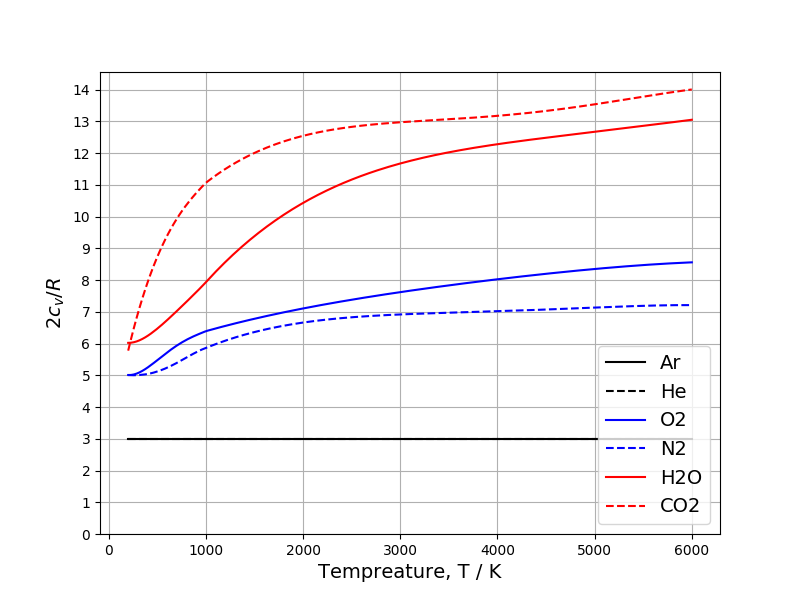
\includegraphics[width=0.97\textwidth]{figures/dof}
\caption{Approximate mean active degrees of freedom in selected ideal gas models}\label{fig:dof}
\end{figure}

For H$_2$O, rigid motion means six degrees of freedom: three coordinates of translation and three axes of rotation.  For diatomic molecules like O$_2$ and N$_2$, however, their symmetry robs them of one of their axes of rotation, so they only exhibit five degrees of freedom at low temperatures.  Since CO$_2$ is also an axisymmetric molecule, it can be seen asymptotically approaching 5 at low temperatures as well.

\subsection{Entropy and enthalpy revisited}\label{sec:ig:hs}

Recall from Section \ref{sec:intro:s} that the entropy of any substance changes like
\begin{align}
T \d s = \d h - v \d p\nonumber.
\end{align}
For the ideal gas, this can be simplified by substituting $R T / p$ for $v$ and integrating to obtain
\begin{align}
s - s_0 = \int c_p(T)\frac{\d T}{T} - R \ln \left( \frac{p}{p^\circ} \right)\label{eqn:ig:s}.
\end{align}
when $p^\circ$ is a reference pressure.  For a perfect gas,
\begin{align}
s - s_0 = c_p \ln\left( \frac{T}{T_0} \right) - R \ln\left( \frac{p}{p^\circ} \right)\label{eqn:pg:s}.
\end{align}
when $T_0$ is a reference temperature.

Evaluating the pressure portion of (\ref{eqn:pg:s}) is straightforward, but it will be seen below that the temperature dependence is more nuanced.  For that reason, it is often treated alone,
\begin{align}
s^\circ(T) = s_0 + \int c_p(T) \frac{\d T}{T},
\end{align}
where $s^\circ$ is the entropy at the reference pressure, $p^\circ$.

An identical approach can be taken for enthalpy, but with an even simpler result.  
\begin{align}
h - h_0 = \int c_p(T) \d T \label{eqn:ig:h}
\end{align}
For a perfect gas,
\begin{align}
h - h_0 = c_p \left(T - T_0\right). \label{eqn:pg:h}
\end{align}

In the NIST-JANAF tables, the specific heat is calculated theoretically from the molecular and atomic structure of each atom, but specific heat is also readily validated by calorimetry.  Entropy's integration constant, $s_0$, is chosen so the values agree with absolute calculations for the species entropy from Boltzmann's statistical model for entropy.  Since no such model exists for enthalpy, $h_0$ is determined by a separate approach described in Section \ref{sec:ig:hf}.

The models in the \texttt{ig} and \texttt{ig2} classes use systems of coefficients to form piece-wise polynomials for $c_p(T)$ instead of using the detailed models recorded in the NIST-JANAF tables.  These are ideal for computational codes because they give good numerical performance, but they are not valid down to the low temperatures included by the original tables.

\subsection{Other properties}

Once $c_p(T)$ is well defined, it is also possible to evaluate internal energy,
\begin{align}
e(T) = h(T) - RT,\label{eqn:ig:e}
\end{align}
constant-volume specific heat,
\begin{align}
c_v(T) = c_p(T) - R,\label{eqn:ig:cv}
\end{align}
specific heat ratio,
\begin{align}
\gamma(T) = \frac{c_p(T)}{c_p(T) - R},\label{eqn:ig:cp}
\end{align}
speed of sound
\begin{align}
a(T) = \sqrt{\gamma(T) R T},\label{eqn:ig:a}
\end{align}
and others.

\subsection{Enthalpy of formation}\label{sec:ig:hf}

When a substance is formed either by nuclear, chemical or phase change, energy is nearly always released or consumed.  This energy is accounted for by a property called the \emph{enthalpy of formation}.  It is the energy required to form a substance, so exothermic reactions have negative enthalpies of formation.  The ideal gas data on which \PM's ideal gas classes do not consider nuclear reactions; only chemical reactions and phase changes.  

One might imagine a reactor with a mixture of reactants flowing in and a mixture of products flowing out.  In the simplest case, we should imagine the products to be made entirely of the substance we wish to study, so the reactants will be only those that are absolutely necessary for forming it and in the correct proportions.
\begin{align}
a \mathrm{A}+ b \mathrm{B} + \ldots \rightarrow \mathrm{A}_a \mathrm{B}_b \ldots
\end{align}

Many such chemical reactions release or consume vast amounts of energy.  Usually, this results in cooling or heating of the substance as it changes.  When heat and work are neither added nor removed from the system, an energy balance mandates an isenthalic process,
\begin{align}
h_\mathrm{reactants} &= h_\mathrm{products}\nonumber\\
a \overline{h}_\mathrm{A} + b \overline{h}_\mathrm{B} + \ldots &= \overline{h}_{\mathrm{A}_a \mathrm{B}_b \ldots}
\end{align}
when $\overline{h}$ is enthalpy in molar units.

This result is often counter intuitive.  Since ideal gas enthalpy is only a function of temperature, it seems like an isenthalpic process should also be isothermal.  However, when chemical or phase changes take place, the enthalpy curves of the products and reactants can be dramatically different.  

Fig. \ref{fig:hf} shows enthalpy curves for a hypothetical set of reactants and products.  Not only may the two have dissimilar slopes, but the curves may have large offsets separating them.  When the process is isenthalpic, these offsets cause temperature changes shown in red.  In the case shown, the reactants have higher enthalpy than the products, so the additional energy is absorbed thermally by the products, causing an increase in temperature.  On a molecular level, the effect is like allowing two magnetic marbles to roll near one another on a flat table.  Even if neither has much velocity to begin with, after they collide, they will be sent off quickly spinning and rolling.  The same happens in an exothermic reaction.

\begin{figure}
\centering
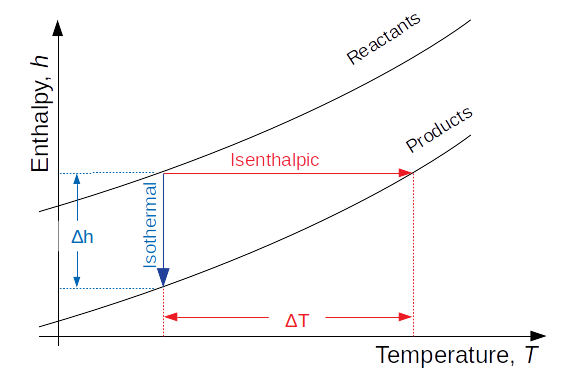
\includegraphics[width=.97\linewidth]{figures/hf}
\caption{Isenthalpic and isothermal reactions on an h-T diagram.}\label{fig:hf}
\end{figure}

If the hypothetical reactor were modified to add or extract heat so that the temperature of the reaction were constant, the process would adopt the vertical blue line instead.  In an isothermal reaction, the amount of thermal energy exhibited by the substance is constant, so any release or consumption of heat will have come from a chemical reaction (including a change in the substance's active degrees of freedom, $f$).  Therefore, the change in enthalpy between the two curves is the enthalpy consumed by the chemical reaction reaction.  

In the diagram, the enthalpy is seen decreasing in order to maintain the temperature, so heat was removed, and the reaction is called exothermic.  For such a reaction, the energy balance would be
\begin{align}
a \overline{h}_\mathrm{A} + b \overline{h}_\mathrm{B} + \ldots + \Delta h &= \overline{h}_{\mathrm{A}_a \mathrm{B}_b \ldots}
\end{align}
Here, the change in enthalpy, $\Delta h$, is positive when energy is added to maintain a constant temperature throughout the reaction, so in the exothermic reaction depicted in fig. \ref{fig:hf}, $\Delta h$ would be negative.  In general $\Delta h$ is also a function of temperature because the properties of the two gas mixtures are not parallel.

The value of $\Delta h(T)$ also depends on which reactants are selected to form the product.  For example, one might select atomic oxygen and atomic hydrogen to form water, but it would be just as valid to chose the more common diatomic hydrogen and oxygen.  These two reactions would exhibit different $\Delta h$ values because the energies of the starting substances are different.  If one wishes to establish a value for $\Delta h$ that is clearly defined and indicates the energy required to form the substance, it is necessary to specify a standard set of ``reference'' substances, relative to which all other substances are derived.

Every element is given exactly one {\bf reference substance}, which may include phase changes (like in the case of the metals).  The enthalpy of formation for the reference substance is arbitrarily declared to be zero at all temperatures, since it is imagined to be a fundamental building block from which compounds are built.

The \emph{enthalpy of formation}, $\Delta_f h$, is the energy consumed by the reaction when all of the reactants are reference substances in the proper proportions to produce the product.

Many of the reference substances are atomic gases or pure liquids and crystals (like argon and aluminum).  Others are selected to be diatomic gases because of their abundance (like hydrogen, oxygen, and nitrogen).

\subsection{Properties of mixtures}\label{sec:ig:mix}

The discussion so far has applied only to properties of pure ideal gases.  The composition of a gas mixture is conventionally defined in either mass or molar quantities of the constituent pure gases.  In this section, we establish methods by which properties can be calculated from the properties of the components.  

In extensive units, a volume, $V$, might contain many individual gas species, each with total mass, $m_i$, or total mole count, $N_i$.  They are related by the pure gas's molecular weight,
\begin{align}
m_i = W_i N_i.
\end{align}

{\bf Mass and mole fractions} are the fractions of a gas composed of a single pure substance. The total mass and count of gas in the volume is merely the sum of all the constituents, $m = \sum m_i$, and $N = \sum N_i$.  These let us more conveniently express the composition in mass and mole fractions, respectively,
\begin{subequations}
\begin{align}
y_i &\equiv \frac{m_i}{\sum m_k}\\
\chi_i &= \equiv \frac{N_i}{\sum N_k}.
\end{align}
\end{subequations}
Note that the fractional quantities, $y_i$ and $\chi_i$, are not dependent on the choice of units for mass or mole count.  Observe that, by definition, $\sum y_i = \sum \chi_i = 1$.

{\bf Mixture density} is the total mass or mole count of all species divided by the volume they occupy.  
\begin{subequations}
\begin{align}
\rho &\equiv \frac{\sum m_i}{V}\\
\overline{\rho} &\equiv \frac{\sum N_i}{V}
\end{align}
\end{subequations}
If $\rho_i$ and $\overline{\rho}_i$ were the densities of constituent $i$ at the same temperature and pressure as the total mixture, then it is important to emphasize that $m_i / V$  and $N_i / V$ are \emph{not} $\rho_i$ and $\overline{\rho}_i$.  That question is addressed below.

{\bf Molecular weight} of a gas mixture has the same definition as the molecular weight of a pure gas; it is the mass per mole count of total gas.  It can be calculated from the constituent molecular weights using either mole fractions or mass fractions,
\begin{subequations}
\begin{align}
W &\equiv \frac{\sum m_i}{\sum N_j}\\
 &= \frac{\sum N_i W_i}{\sum N_j}\nonumber\\
 &= \sum \chi_i W_i\label{eqn:w:x}\\
 &= \frac{\sum m_i}{\sum m_j / W_j}\nonumber\\\
 &= \left(\sum \frac{y_j}{W_j} \right)^{-1}.\label{eqn:w:y}
\end{align}
\end{subequations}

{\bf Partial pressure}, $p_i$, is the pressure force exerted on a surface due only to collisions of a single constituent, $i$.  Section \ref{sec:ig:iglaw} will help understand what is meant by this idea.  It is the pressure force that would be measured if all other constituent gases were removed.  
\begin{align}
p_i &\equiv \frac{N_i}{V} R_u T \nonumber\\
 &= \chi_i \frac{N}{V} R_u T \nonumber\\
 &= \chi_i \overline{\rho} R_u T
\end{align}

The same pressure may be calculated from mass fraction,
\begin{align}
p_i &= \frac{N_i}{V} R_u T \nonumber\\
 &= \frac{m_i}{W_i V} \rho R_u T \nonumber\\
 &= y_i \rho R_i T
\end{align}
The ideal gas constant, $R_i$, is the mass-based gas constant for only that constituent, $R_i = R_u / W_i$.

{\bf Total pressure}, $p$, is the pressure force actually experienced by a surface due to all of the constituent gases.  By definition, 
\begin{align}
p &= \sum p_i \nonumber\\
 &= \overline{\rho} R_u T
\end{align}
Observe, also, that 
\begin{align}
\chi_i = \frac{p_i}{p}.
\end{align}

The total pressure can also be calculated in terms of mass density.  Using (\ref{eqn:w:y}),
\begin{align}
p &= \sum p_i \nonumber\\
 &= \sum y_i \rho R_i T\nonumber\\
 &= \sum \frac{y_i}{W_i} \rho R_u T\nonumber\\
 &= \rho R T.
\end{align}
The total mixture gas constant appears naturally.

{\bf The mixture gas constant}, $R$, appears naturally when calculating total pressure from total mass density, and it is calculated in precisely the same way as a pure gas constant, but the mixture molecular weight is used instead,
\begin{subequations}
\begin{align}
R &\equiv \frac{R_u}{W}\\
 &= \frac{R_u}{\sum \chi_i W_i}\nonumber\\
 &= \left( \frac{\chi_i}{R_i} \right)^{-1}\\
 &= R_u \sum \frac{y_i}{W_i}\nonumber\\
 &= \sum y_i R_i
\end{align}
\end{subequations}

{\bf Densities} can be calculated from the same properties of the component species using the ideal gas law.  For mass density,
\begin{subequations}
\begin{align}
\rho &= \frac{p}{R T}\nonumber\\
 &= \frac{p}{\sum y_i R_i T}\nonumber\\
 &= \left(\sum \frac{y_i}{\rho_i(T,p)} \right)^{-1}\\
 &= \frac{p}{\left(\sum \chi_i / R_i\right)^{-1} T}\nonumber\\
 &= \sum \chi_i \rho_i(T,p)
\end{align}
\end{subequations}

For molar density, no such complexity is needed, since the universal gas constant is the same for all gases,
\begin{align}
\overline{\rho} &= \frac{p}{R_u T}\nonumber
\end{align}

{\bf Internal energy, enthalpy, entropy, and other bulk properties} are merely the sum of all the values contributed by each of the constituent gases.  By definition in an ideal gas, the presence of other gases do not affect the behavior of each of the pure constituents.  Therefore, a bulk property may be calculated from the properties of the pure substances under equivalent temperature and pressure,
\begin{align}
\left(\sum m_j\right) \phi(T,p) &= \sum m_i \phi_i(T,p)\nonumber\\
\left(\sum N_j \right) \overline{\phi}(T,p) &= \sum N_i \overline{\phi}_i(T,p)\nonumber
\end{align}
Therefore, 
\begin{align}
\phi(T,p) &= \sum y_i \phi_i(T,p)\nonumber\\
\overline{\phi}(T,p) &= \sum \chi_i(T,p) \overline{\phi}_i\nonumber
\end{align}
This is hardly a proof, but it is sufficient for the scope of this document to assert that it is true for bulk properties.

This identity may be applied to internal energy, enthalpy, entropy, and all the properties derived from them, so
\begin{subequations}
\begin{align}
e(T) &= \sum y_i e_i(T)\\
h(T) &= \sum y_i h_i(T)\\
s(T,p) &= \sum y_i s_i(T,p_i)
\end{align}
\end{subequations}
and
\begin{subequations}
\begin{align}
\overline{e}(T) &= \sum \chi_i \overline{e}_i(T)\\
\overline{h}(T) &= \sum \chi_i \overline{h}_i(T)\\
\overline{s}(T,p) &= \sum \chi_i \overline{s}_i(T,p_i).
\end{align}
\end{subequations}


\section{The ideal gas collection}

There are several classes that implement various data models for ideal gas properties.  Their interfaces are all standardized so that very little difference should be apparent to the user, except that the ideal gas mixture class has some extra methods associated with its composition.

All property methods accept any two of temperature, density, or pressure to specify the state.

\subsection{The Shomate equation: \texttt{ig}}\label{sec:ig:ig}

\PM's \texttt{ig} class is built on the Shomate equation for constant-pressure specific heat $c_p$.  This is the formulation used by the NIST webbook \cite{nist:webbook}.  Despite the wise range of substances represented, it has the advantage of using a simple standard piece-wise formulation for specific heat.  However, it does suffer from certain limitations.

The Shomate equation takes the form
\begin{align}
\theta &= \frac{T}{T_s}\\
c_p(t) &= c_0 + c_1 \theta + c_2 \theta^2 + c_3 \theta^3 + \frac{c_4}{\theta^2},
\end{align}
where the scaling temperature, $T_s$ is 1000K for all species.  The decision to scale the temperature by a large value has the effect of scaling $\tau$ so that it will not be much larger than 5 or 6.  That helps reduce numerical errors in high-order polynomials.

Because of its simplicity, the Shomate equations lack the degrees of freedom to express specific heat over wide ranges, so data are usually given in piece-wise formulations.  For example, tungsten dioxide (WO$_2$), has a set of coefficients for $298\mathrm{K} \le T < 1100\mathrm{K}$ and $1100\mathrm{K} \le T \le 6000\mathrm{K}$.

The enthalpy can be explicitly calculated from (\ref{eqn:ig:h}),
\begin{align}
h(T) &= h_0 + \int c_p(T) \d T \nonumber\\
 &= h_0 + T_s \int c_p(\theta) \d \theta \nonumber\\
 &= T_s \left(c_0 \theta + \frac{c_1}{2} \theta^2 + \frac{c_2}{3} \theta^3 + \frac{c_3}{4} \theta^4 - \frac{c_4}{\theta} + c_5 \right).
\end{align}
It is important to emphasize that $h_0$ is not the same as the enthalpy of formation, $\Delta h^\circ_f$.  Instead, it is merely an integration constant, which can be alternately expressed as a new coefficient, $c_5$.

Because of the temperature term in the denominator, no multiple of $T_s$ appears in entropy when the integration is changed to $\theta$,
\begin{align}
s^\circ(T) &= s_0 + \int \frac{c_p(T)}{T}\d T\nonumber\\
 &= s_0 + \int \frac{c_p(\theta)}{\theta}\d \tau\nonumber\\
 &= c_0 \ln \theta + c_1 \theta + \frac{c_2}{2} \theta^2 + \frac{c_3}{3} \theta^3 -\frac{c_4}{2\theta^2} + c_6\\
s(T,p) &= s^\circ(T) - R \ln \left( \frac{p}{p^\circ} \right)\nonumber
\end{align}
Just like in the enthalpy integral, a new coefficient, $c_6$, has been introduced to represent the integration constant.

Internal energy is readily calculated from the definition of enthalpy in (\ref{eqn:ig:h}),
\begin{align}
e(T) &= h(T) - RT
\end{align}
There is a similarly simple relationship to determine constant-volume specific heat and specific heat ratio,
\begin{align}
c_v(T) &= c_p(T) - R\\
\gamma(T) &= \frac{c_p(T)}{c_p(T)-R}
\end{align}

Table \ref{tab:class:ig} lists the data elements that define the \texttt{ig} class.  For more information on how \texttt{.hpd} files are stored, see Section \ref{sec:regdat:data}.  Most of the essential data elements are self explanatory, but the coefficients and temperature limits must have compatible sizes.  Even though the \texttt{ig} class only uses seven coefficients, there are eight provided in the NIST data sets.  If there are $N$ sets of coefficients defined over $N$ temperature ranges, there must be $N$ arrays of eight coefficients and $N+1$ temperature limit values.
5
For example, in a data set with two temperature ranges, the following would define a data set valid between \texttt{<T0>} and \texttt{<T2>}, and the transition between the two piece-wise data sets is at \texttt{<T1>}.
\begin{lstlisting}[language=Python]
"Tlim":[<T0>, <T1>, <T2>]
"C":[
  [ <c0>, <c1>, <c2>, <c3>, <c4>, <c5>, <c6>, <c7> ],
  [ <c0>, <c1>, <c2>, <c3>, <c4>, <c5>, <c6>, <c7> ],
]
\end{lstlisting}

\begin{table}
\centering
\caption{HPD data file elements for the \texttt{ig} class}\label{tab:class:ig}
\begin{tabular}{|ccp{2.5in}|}
\hline
Name & Type & Description\\
\hline
\texttt{id} & \texttt{str} & Unique substance identifier string\\
\texttt{class} & \texttt{='ig'} & Class identifier string\\
\texttt{doc} & \texttt{str} & Documentation string\\
\hline
\texttt{atoms} & \texttt{dict} & Keys are elemental atoms, and values are their integer quantities in the substance.\\
\texttt{mw} & \texttt{float} & The molecular weight.\\
\texttt{Tlim} & \texttt{list} & A sorted list of $N+1$ floating point temperatures.  Middle values define the boundaries between piece-wise coefficient ranges.  High and low values define the limits of the model.\\
\texttt{C} & nested \texttt{list} & The value, $C[i][j]$, corresponds to coefficient $c_j$ in the temperature interval \texttt{Tlim[i]} to \texttt{Tlim[i+1]}.\\
\hline
\texttt{TAB} & nested \texttt{list} & Optional table of truth values published by NIST used for validation\\
\hline
\end{tabular}
\end{table}


\subsection{The NASA polynomial: \texttt{ig2}}\label{sec:ig:ig2}

The so-called ``NASA polynomials'' are a piece-wise empirical formulation to the specific heat of an ideal gas.  They are taken from \cite{mcbride:1993} predate the latest formulation of the NIST-JANAF tables, and are even used for reference.  Unlike the Shomate equation, there is no $1/t^2$ term, there is no attempt to scale temperature prior to evaluating the polynomial, and properties are scaled with respect to the ideal gas constant.

\begin{align}
c_p(T) = R\left(c_0 + c_1 T + c_2 T^2 + c_3 T^3 + c_4 T^4\right)
\end{align}

There are nearly identical formulations for enthalpy,
\begin{align}
h(T) = R \left(c_0 T + \frac{c_1}{2} T^2 + \frac{c_2}{3} T^3 + \frac{c_3}{4} T^4 + \frac{c_4}{5}T^5 + c_5 \right),
\end{align}
and entropy
\begin{align}
s^\circ(T) = R \left(c_0 \ln(T) + c_1 T + \frac{c_2}{2} T^2 + \frac{c_3}{3} T^3 + \frac{c_4}{4} T^4 + c_6\right).
\end{align}
Here, just as in the Shomate equations, $c_5$ and $c_6$ are introduced as integration constants in enthalpy and entropy.

Internal energy is readily calculated from the definition of enthalpy in (\ref{eqn:ig:h}),
\begin{align}
e(T) &= h(T) - RT\nonumber\\
\end{align}
There is a similarly simple relationship to determine constant-volume specific heat and specific heat ratio,
\begin{align}
c_v(T) &= c_p(T) - R\\
\gamma(T) &= \frac{c_p(T)}{c_p(T)-R}
\end{align}

There is some overlap in the species offered by the two classes.  A mild preference has been given to the older NASA polynomials for two reasons:
\begin{itemize}
\item Most of the NASA models have wider ranges of validity than the Shomate models.
\item Some of the Shomate data have been found to suffer from discontinuity errors at the piecewise boundaries.
\end{itemize}
Otherwise, the two have been found to be sufficiently equivalent that most users will not find a reason to wonder.

Table \ref{tab:class:ig2} lists the data elements that define the \texttt{ig2} class.  For more information on how \texttt{.hpd} files are stored, see Section \ref{sec:regdat:data}.  Most of the essential data elements are self explanatory, but the coefficients and temperature limits must have compatible sizes.  Even though the \texttt{ig2} class only uses seven coefficients, there are eight provided in the NIST data sets.  If there are $N$ sets of coefficients defined over $N$ temperature ranges, there must be $N$ arrays of eight coefficients and $N+1$ temperature limit values.

For example, in a data set with two temperature ranges, the following would define a data set valid between \texttt{<T0>} and \texttt{<T2>}, and the transition between the two piece-wise data sets is at \texttt{<T1>}.
\begin{lstlisting}[language=Python]
"Tlim":[<T0>, <T1>, <T2>]
"C":[
  [<c0>, <c1>, <c2>, <c3>, <c4>, <c5>, <c6>, <c7>],
  [<c0>, <c1>, <c2>, <c3>, <c4>, <c5>, <c6>, <c7>],
]
\end{lstlisting}

\begin{table}
\centering
\caption{HPD data file elements for the \texttt{ig2} class}\label{tab:class:ig2}
\begin{tabular}{|ccp{2.5in}|}
\hline
Name & Type & Description\\
\hline
\texttt{id} & \texttt{str} & Unique substance identifier string\\
\texttt{class} & \texttt{='ig2'} & Class identifier string\\
\texttt{doc} & \texttt{str} & Documentation string\\
\hline
\texttt{atoms} & \texttt{dict} & Keys are elemental atoms, and values are their integer quantities in the substance.\\
\texttt{pref} & \texttt{float} & Reference pressure in Pascals\\
\texttt{mw} & \texttt{float} & The molecular weight.\\
\texttt{Tlim} & \texttt{list} & A sorted list of $N+1$ floating point temperatures: Middle values define the boundaries between piece-wise coefficient ranges.  High and low values define the limits of the model.\\
\texttt{C} & nested \texttt{list} & The value, $C[i][j]$, corresponds to coefficient $c_j$ in the temperature interval \texttt{Tlim[i]} to \texttt{Tlim[i+1]}.\\
\hline
\end{tabular}
\end{table}

\subsection{The ideal gas mixture: \texttt{igmix}}\label{sec:ig:igmix}

The \PM\ ideal gas mixture class defines methods to calculate properties of a static mixture of ideal gases.  For improved computational efficiency, properties like the mixture molecular weight, mole fractions, and mass fractions, are calculated ahead of time and stored in class instances for later use.

Section \ref{sec:ig:mix} already shows how properties of a mixture can be calculated from the properties of the constituent gases.  The implementation of all but entropy is quite straightforward.  In all of the ideal gas codes, the entropy at the reference pressure, $s^\circ$, is calculated in a separate efficient internal method.  For that reason, the \texttt{igmix} class calls on these methods directly and then treats the pressure dependence separately.

When calculating in molar units,
\begin{align*}
\overline{s}(T,p) &= \sum \chi_i \overline{s}(T, p_i)\\
 &=\sum \chi_i\ \overline{s}^\circ_i(T) - \sum \chi_i R_u \ln\left(\frac{p \chi_i}{p^\circ_i}\right),
\end{align*}
where $p_i$ is the partial pressure of constituent $i$ and $p^\circ_i$ is the reference pressure of constituent $i$.

The partial pressure is merely $p \chi_i$, but the reference pressure for each substance may vary depending on the data source.  We deal with this in the following way.
\begin{align*}
\sum \chi_i \ln\left(\frac{p \chi_i}{p^\circ_i}\right) &= \sum \chi_i \left( \ln p + \ln \chi_i - \ln p^\circ_i \right)\\
&= \left( \ln p - \sum \chi_i \ln p^\circ_i\right) + \sum \chi_i \ln \chi_i
\end{align*}
When
\begin{align}
p^\circ_\mathrm{mix} &= \exp\left(\sum \chi_i \ln p^\circ_i \right)\\
s_\mathrm{mix} &= -R_u \sum \chi_i \ln \chi_i,
\end{align}
the enthalpy is calculated by
\begin{align*}
\overline{s}(T,p) &= \overline{s}_\mathrm{mix} + \sum \chi_i\ \overline{s}^\circ_i(T) - R_u \ln\left( \frac{p}{p^\circ_\mathrm{mix}} \right),
\end{align*}

The new reference pressure, $p^\circ_\mathrm{mix}$, is a log-weighted average of the constituent reference pressures.  In the event that they are all the same, the mixture reference pressure is also the same.  

Neither a function of temperature nor pressure, the entropy of mixing, $\overline{s_\mathrm{mix}}$, is a constant that represents the entropy created by dispersing constituent gases into one another.  Note that it is added to the entropy that would be calculated from the pure constituents.

\begin{table}
\centering
\caption{HPD data file elements for the \texttt{igmix} class}\label{tab:class:igmix}
\begin{tabular}{|ccp{2.5in}|}
\hline
Name & Type & Description\\
\hline
\texttt{id} & \texttt{str} & Unique substance identifier string\\
\texttt{class} & \texttt{='igmix'} & Class identifier string\\
\texttt{doc} & \texttt{str} & Documentation string\\
\hline
\texttt{bymass} & \texttt{bool} & Indicates whether contents are listed by mass or by mole count\\
\texttt{contents} & \texttt{dict} & Specifies the mixture composition: Keys are pure ideal gas id strings, values are quantities.  The quantities will be normalized after load, so they do not need to add to one.\\
\hline
\end{tabular}
\end{table}



\end{document}
